\documentclass[12pt,a4paper]{article}

% --------------------------------------------------------
%              PACKAGES ET CONFIGURATION
% --------------------------------------------------------
%              PACKAGES ET CONFIGURATION
% --------------------------------------------------------
\usepackage[utf8]{inputenc}
\usepackage[T1]{fontenc}
\usepackage[french]{babel}
\usepackage{geometry}
\geometry{margin=1in}
\usepackage{setspace}
\onehalfspacing
\usepackage{csquotes}
\usepackage{graphicx}
\usepackage{pdflscape}
\usepackage{float} 
\DeclareUnicodeCharacter{2009}{\,}  
\DeclareUnicodeCharacter{202F}{\,}

\usepackage[dvipsnames]{xcolor} % Active les couleurs étendues
\usepackage[
    colorlinks=true,
    linkcolor=black,
    urlcolor=OliveGreen,
    citecolor=black,
    pdfauthor={Naromba Condé, Tunwend-raabo Fahîma Carmen DABO, Abdelghafour Rahmouni},
    pdftitle={IFT3150 - Rapport final : Pique-Me}
]{hyperref}

\usepackage{enumitem}
\setlist[itemize]{leftmargin=1.5em}
\setlist[enumerate]{leftmargin=1.5em}

% --------------------------------------------------------
%                      COMMANDES TITRE
% --------------------------------------------------------
\newcommand{\university}{\textsc{Université de Montréal}}
\newcommand{\mainTitle}{\textbf{IFT3150 — Rapport final}}
\newcommand{\projectSubtitle}{\large\emph{Pique-Me :  Montréal à la carte}}
\newcommand{\authorsBlock}{%
  Par\\[0.75em]
  \textbf{Tunwend-raabo Fahîma Carmen DABO } (20266362)\\
  \textbf{Abdelghafour Rahmouni} (20246224)\\
  \textbf{Naromba Condé} (20251772)
}
\newcommand{\presentedTo}{Travail présenté à \textbf{Gena Han}\\[0.25em]
Dans le cadre du cours IFT3150 : Projet d'informatique}
\newcommand{\dateBlock}{\today}

% --------------------------------------------------------
%                        DOCUMENT
% --------------------------------------------------------


\begin{document}
\pagenumbering{gobble}

% ---------- PAGE DE GARDE ----------
\begin{titlepage}
  \centering
  \vspace*{1.5cm}
  {\Large \university\par}
  \vfill
  {\Large \mainTitle\par}
  \vspace{0.75cm}
  {\projectSubtitle\par}
  \vfill
  {\authorsBlock\par}
  \vfill
  {\presentedTo\par}
  \vspace{0.75cm}
  {\dateBlock\par}
\end{titlepage}

% ---------- TABLE DES MATIÈRES ----------
\clearpage
\tableofcontents
\clearpage
\pagenumbering{arabic}

% =========================================================
% 1. INTRODUCTION
% =========================================================
\section{Introduction}

\subsection*{Contexte}
À Montréal, les parcs font partie intégrante du quotidien : lieux de détente,
de sport, de rencontres familiales ou d'événements de quartier.
Lors des beaux jours, ces espaces deviennent des pôles d'activité
majeurs. Pourtant, il n'existe toujours pas de moyen numérique unique
et fiable pour connaître les différents espaces, se renseigner sur l'accessibilité ou la
disponibilité d'un équipement avant de s'y rendre.

Il existe l'initiative \textit{Accès nature} permet de 
réserver gratuitement des accès dans plus de trente parcs régionaux via le site \href{https://www.parq.ca/ressources/acces-nature}{toutlemondedehors.ca}, 
mais cette ressource est encore méconnue du grand public et est plus centrée sur les parcs régionaux du Québec.

\subsection*{Problématique}
Les usagers se posent invariablement les mêmes questions :
\textit{Le parc autorise-t-il les barbecues ? Est-il accessible aux personnes à mobilité réduite ?
Reste-t-il des emplacements libres ? Comment trouver le parc qui répond le mieux à nos préférences ?}  
Ces interrogations sont loin d'être anodines. 

Par exemple, à Montréal, l'utilisation de barbecues est 
autorisée dans certains parcs comme Angrignon, Jarry ou La Fontaine, mais elle dépend du type d'appareil 
(charbon ou propane) et de la signalisation sur place. De plus, des barbecues collectifs sont disponibles 
dans certains lieux, mais peu de gens savent où les trouver dans le parc.


En somme, les informations sont dispersées, parfois incomplètes ou obsolètes, ce qui crée une planification laborieuse et une expérience 
parfois décevante. Une centralisation intelligente et interactive de ces données améliorerait considérablement l'expérience des usagers.


\subsection*{Proposition}
\href{https://github.com/Abdou2111/Pique-me}{\textbf{Pique-Me}} vise à concentrer toutes ces données dans une
application mobile intuitive : carte interactive, fiches synthétiques de
parcs, filtres personnalisés, réservation d'emplacements ou d'activités,
système d'avis/badges et notifications d'événements.


\subsection*{Objectifs}
\vspace{-0.25\baselineskip}
\begin{itemize}[nosep]
  \item Concevoir une \textbf{interface mobile fluide} listant les parcs,
        leurs équipements et les activités qui y sont proposées.
  \item \textbf{Implémenter la réservation} d'emplacements/activités
        avec double confirmation et annulation automatique.
  \item Développer une \textbf{dimension communautaire} (favoris, avis,
        badges).
  \item Satisfaire des exigences de \textbf{sécurité, performance,
        accessibilité} et disponibilité.
\end{itemize}

\clearpage
\section{Analyse des besoins et étude préliminaire}

\subsection{Démarche générale}
Le recueil des besoins a débuté dans le cadre du cours
\textbf{IFT2905 – Interfaces personne-machine}, où \emph{Pique-Me} a été
choisi comme projet de session. Nous avons ensuite :
\begin{itemize}
  \item réalisé des entretiens informels avec des amis et proches
        utilisateurs réguliers des parcs montréalais ;
  \item analysé nos propres expériences de planification de pique-niques
        et d'activités extérieures (difficultés et attentes).
\end{itemize}
Les résultats ont été triés puis convertis en
exigences fonctionnelles et non fonctionnelles.

%-------------------------------------------------------------------
\subsection{Exigences fonctionnelles}
\begin{enumerate}[label=\textbf{F\arabic*}.]
  \item \textbf{Authentification \& profil}  
        \begin{itemize}
          \item Inscription par courriel/Google ou usage invité ;
          \item Initialisation des préférences (activités, équipements) ;
          \item Consultation, modification, suppression du compte.
        \end{itemize}
  \item \textbf{Recherche \& découverte de parcs}  
        \begin{itemize}
          \item Barre de recherche (adresse/nom) avec  complétion automatique ;
          \item Filtres dynamiques (équipements, BBQ, activités proposées, etc.) ;
          \item Carte interactive dynamique : la carte suit la position de l'utilisateur et affiche progressivement les parcs (pins) visibles selon le niveau de zoom.

        \end{itemize}
  \item \textbf{Réservation}  
        \begin{itemize}
          \item Sélection d'emplacement ou d'activité via un calendrier ;
          \item Double confirmation (avant/après début) ;
          \item Annulation automatique si non-confirmation 60 min après le debut de la réservation.
        \end{itemize}
\item \textbf{Interaction communautaire} \\
\hspace*{1.5em}\textbf{Avis post-visite :} L'utilisateur sélectionne un ou plusieurs badges pour recommander le parc selon son expérience (ex.~plein air, famille, détente). Il peut aussi ajouter un commentaire et joindre des photos. Si un badge atteint un certain seuil de votes, une médaille (bronze, argent ou or) est attribuée au parc pour ce badge.

\item \textbf{Favoris et  notifications} \\
L'utilisateur peut ajouter ou retirer un parc de sa liste de favoris, qu'il peut consulter à tout moment pour retrouver rapidement ses lieux préférés. Des notifications personnalisées sont envoyées en fonction de ses activités : rappels de réservation, invitations à répondre à un sondage post-visite, ou encore annonces d'événements organisés dans les parcs qu'il a mis en favori.

\end{enumerate}

\subsection{Exigences non fonctionnelles}
\begin{description}
  \item[Performance] L'application doit être rapide : la plupart des requêtes doivent s'afficher en moins de 3 secondes. L'écran d'accueil doit être mis à jour automatiquement en fonction des préférences et de la localisation de l'utilisateur.
  
  \item[Sécurité] Les connexions doivent être sécurisées, et les mots de passe bien protégés. Seules les personnes autorisées peuvent accéder aux données.
  
  \item[Compatibilité] L'application doit bien fonctionner sur les téléphones Android et iPhone, avec des écrans de tailles standards.
  
  \item[Accessibilité] L'interface doit être facile à utiliser, même pour les personnes ayant des difficultés visuelles ou motrices (bons contrastes, navigation simple, etc.).
  
  \item[Fiabilité] L'application doit fonctionner sans planter, et rester disponible au moins 99\,\% du temps.
  
  \item[Confidentialité] Seules les informations nécessaires sont demandées. L'utilisateur peut à tout moment effacer son compte ou ses données s'il le souhaite.
\end{description}


%-------------------------------------------------------------------
\subsection{Méthodologie}

Pour développer notre application \textit{Pique-Me}, nous avons choisi une approche Agile en utilisant la méthode Scrum. Cette méthode permet d'avancer de manière itérative, en découpant le projet en sprints de une semaines. Chaque sprint se concentre sur un ensemble clair de fonctionnalités à livrer, facilitant la planification, l'adaptation continue et l'évaluation du progrès.


Cette approche nous permet de rester flexibles, réactifs aux retours, et de garantir un produit fonctionnel à chaque étape importante du projet.

\clearpage
% =========================================================
% 3. CONCEPTION
% =========================================================
\section{Conception}

\subsection{Architecture du système}

L'application \textit{Pique-Me} repose sur une architecture en trois couches, chaque composant ayant un rôle spécifique dans le traitement des données et l'interaction utilisateur.

\begin{itemize}
  \item \textbf{Frontend :} développé avec React Native et Expo, il s'agit de l'interface utilisateur de l'application mobile (Android/iOS). Elle permet de :
  \begin{itemize}
    \item rechercher des parcs et filtrer les résultats,
    \item réserver des emplacements ou activités,
    \item consulter ses favoris et gérer son compte.
  \end{itemize}

  \item \textbf{Backend :} basé sur Node.js et Express, il traite les requêtes envoyées par l'application. Il centralise la logique métier, vérifie les disponibilités, contrôle les réservations, interroge Firebase et l'API de la Ville de Montréal.

  \item \textbf{Données :} deux sources principales :
  \begin{itemize}
    \item \textbf{Firebase :} stocke les utilisateurs, réservations, favoris, avis, etc.
    \item \textbf{API de la Ville de Montréal :} fournit les données officielles des parcs (équipements, localisation, règlements). Ces données ont été extraites et stockées dans Firebase.
  \end{itemize}
\end{itemize}

\begin{figure}[H]
  \centering
  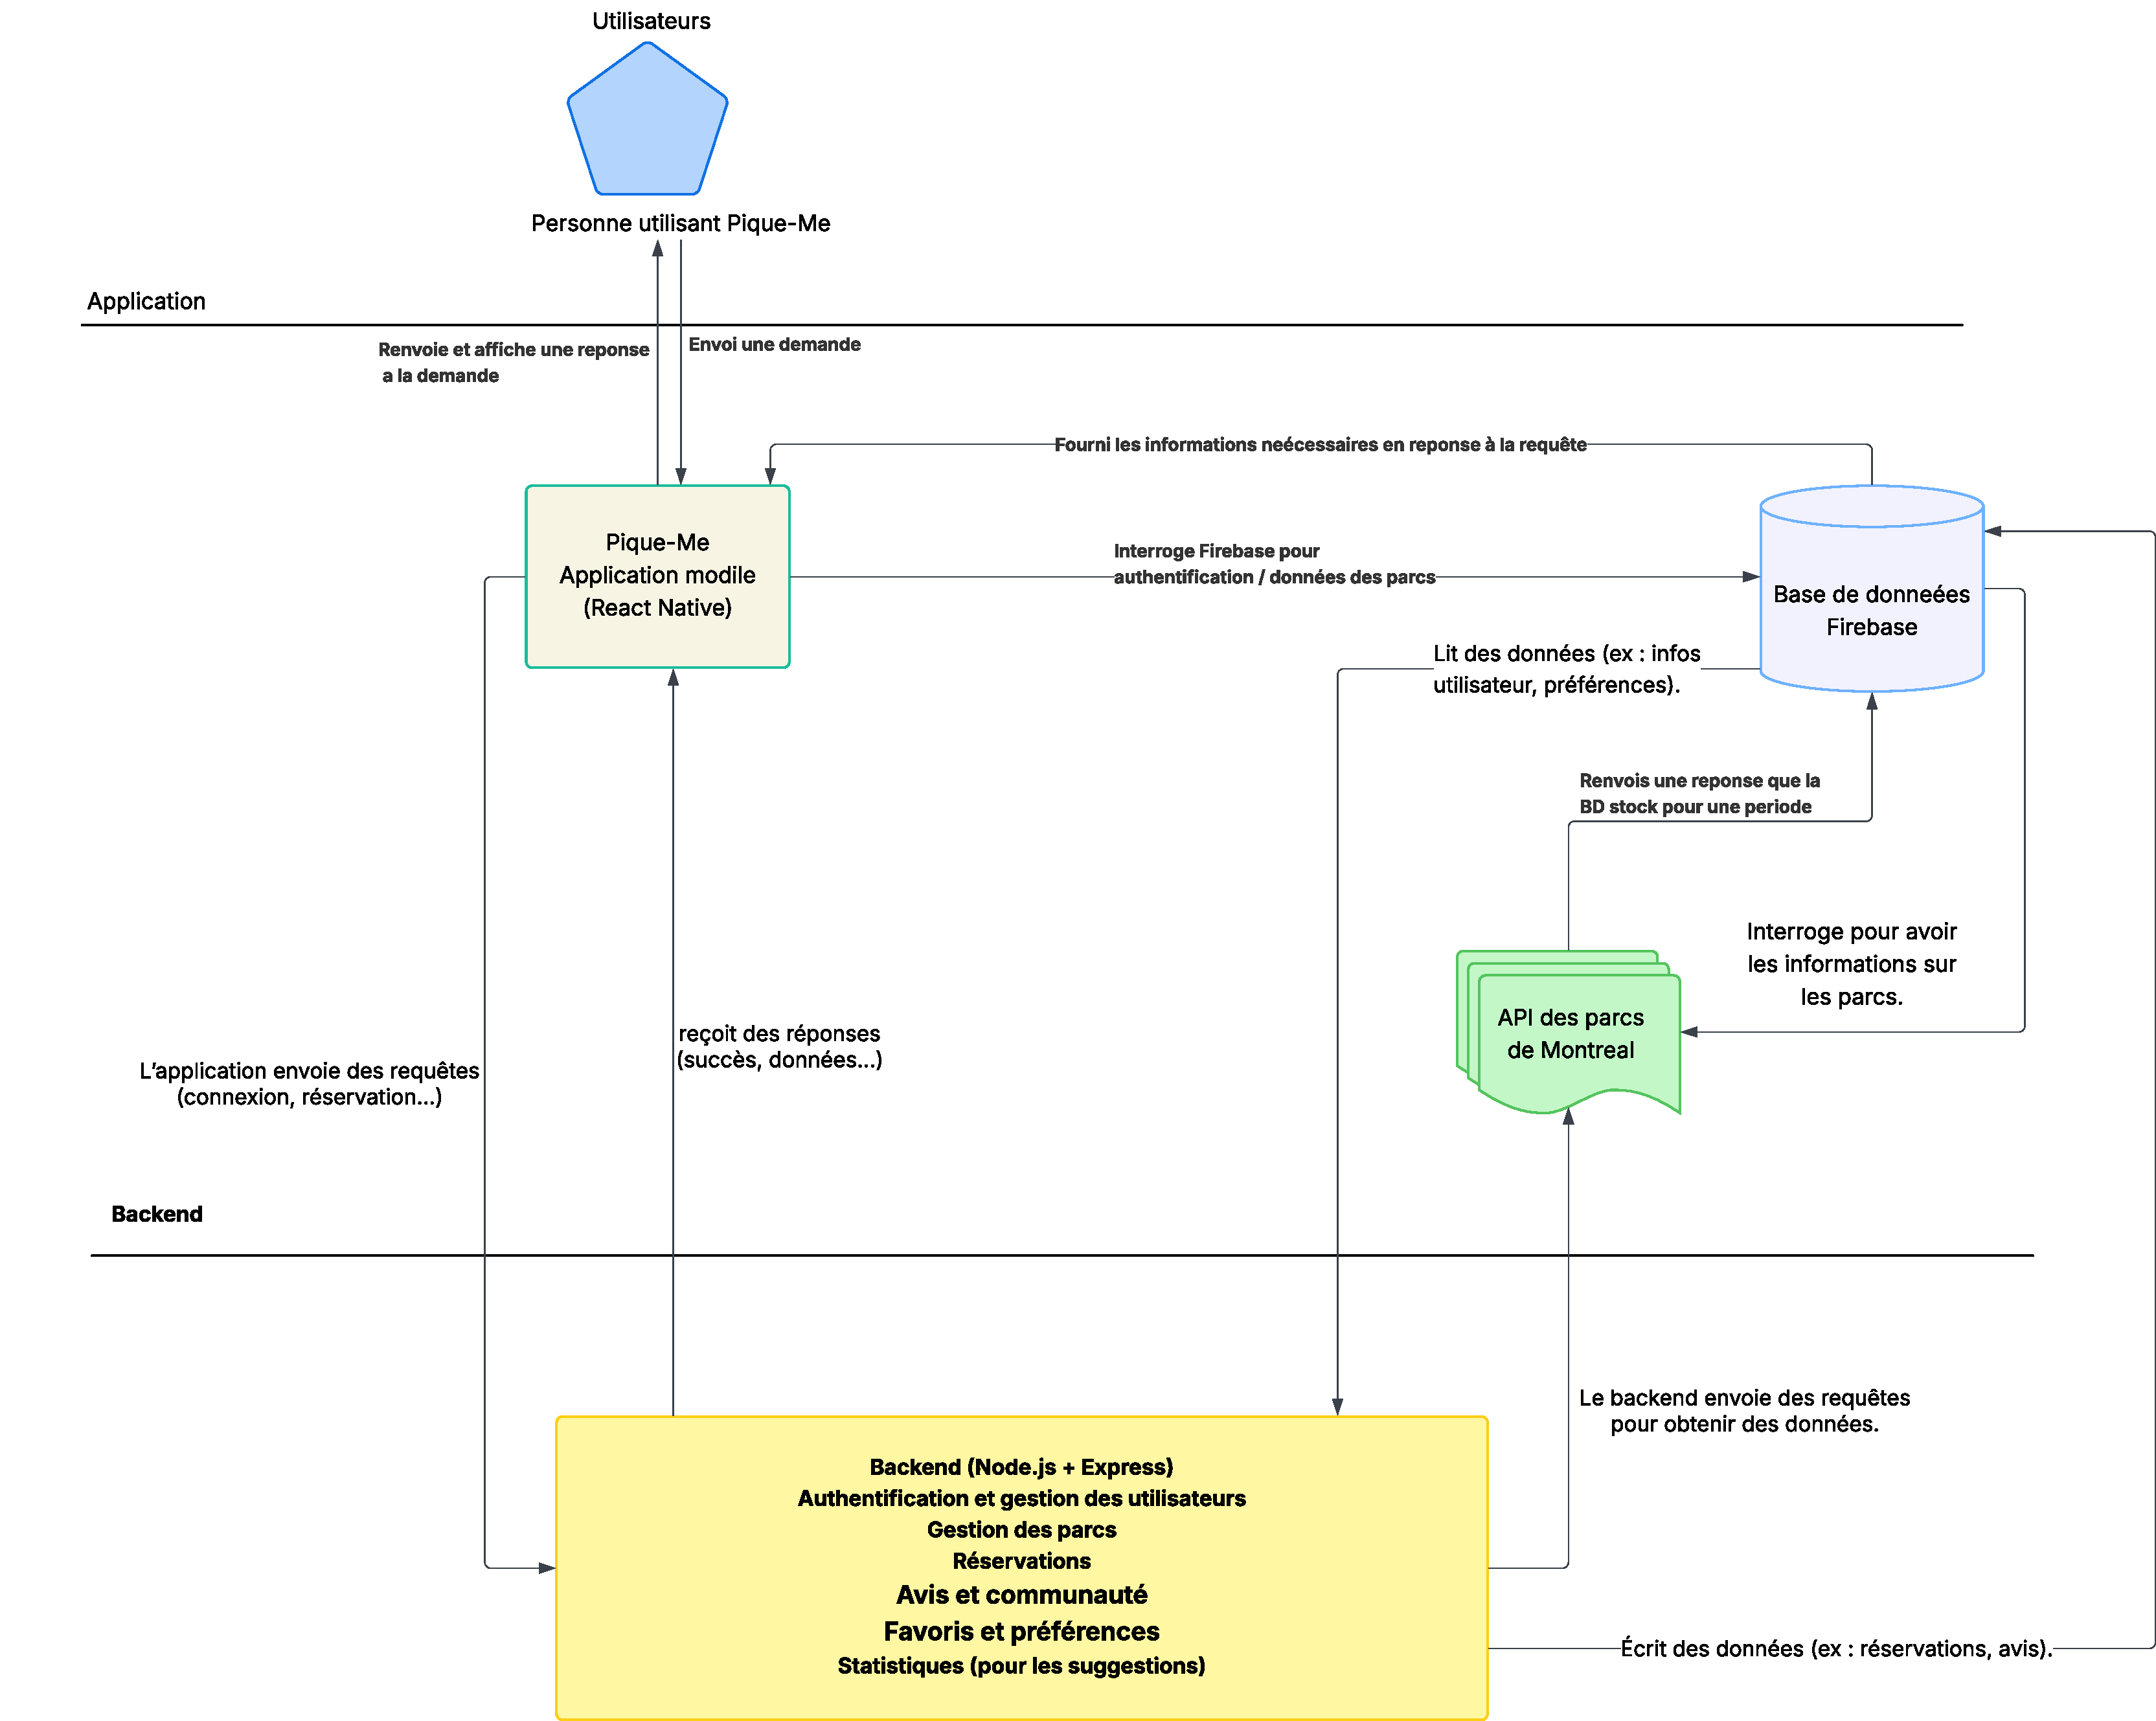
\includegraphics[width=0.9\linewidth]{attachments/architecture.pdf}
  \caption{Architecture logique de l'application Pique-Me.}
\end{figure}

\subsection{Modèle de données}

Le schéma suivant montre le modèle de données UML utilisé pour l'application Pique-Me.
Il présente les éléments importants de l'application, comme les utilisateurs, les parcs, les réservations, les événements, les équipements, les avis et les photos.
On y voit aussi comment ces éléments sont liés entre eux. 

\begin{figure}[H]
  \centering
  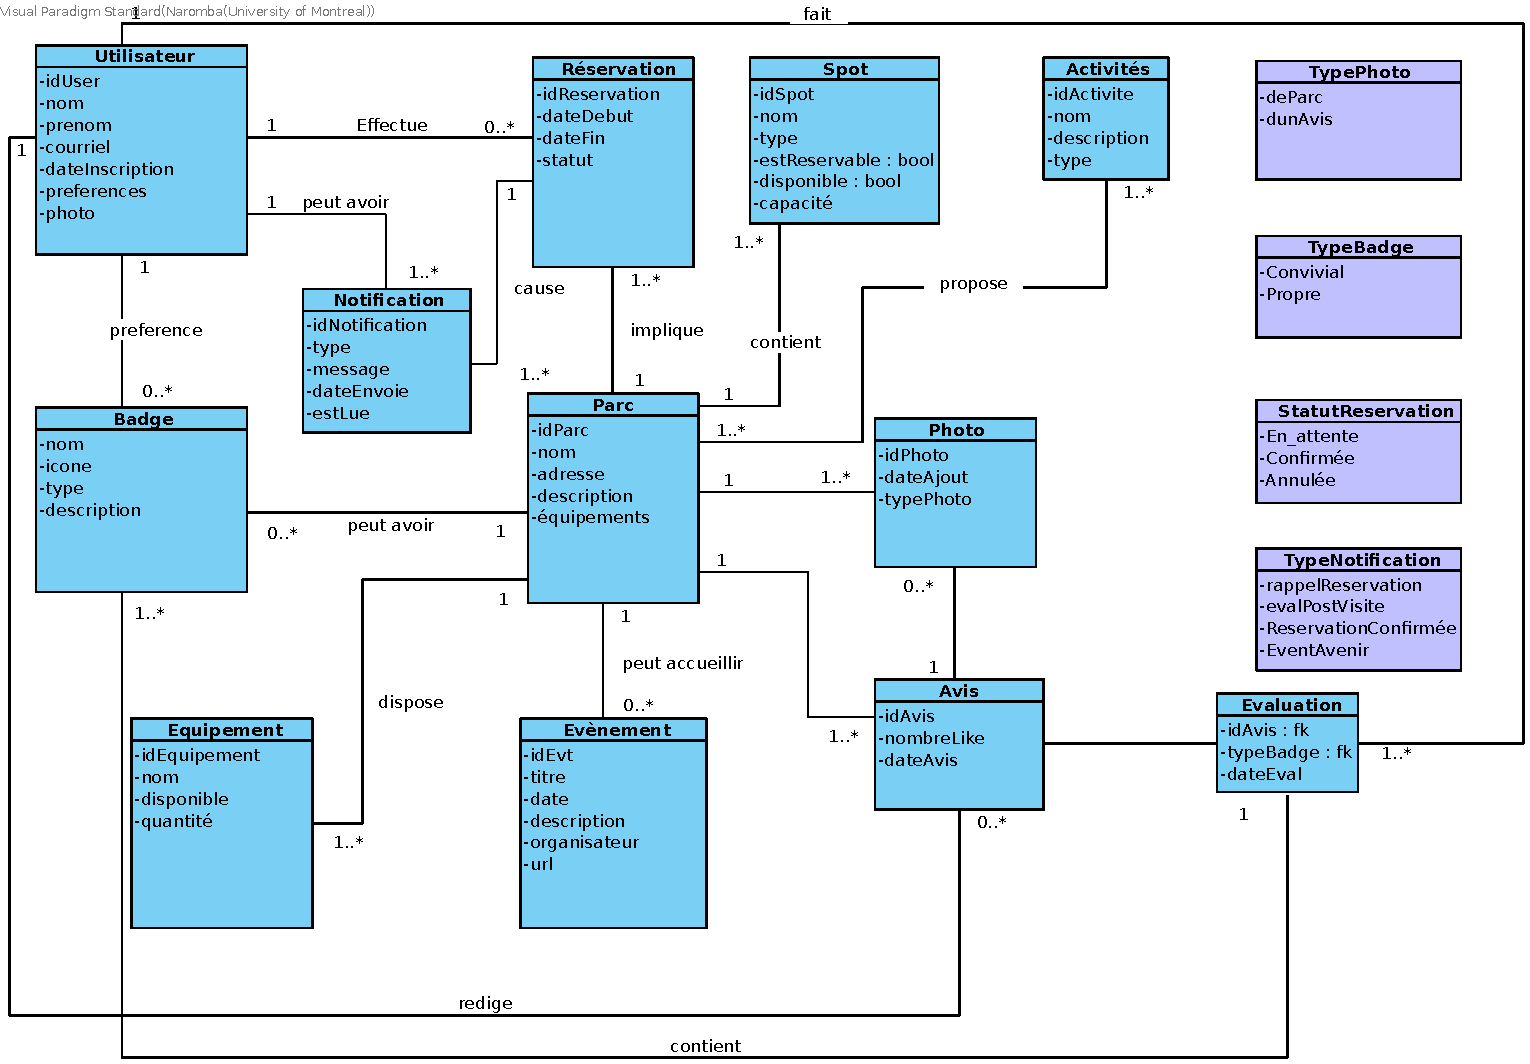
\includegraphics[width=0.9\linewidth]{attachments/donnee.pdf}
  \caption{Diagramme Entité–Association de Pique-Me.}
\end{figure}


\subsection{Choix technologiques et justifications}

\paragraph{\textbf{\href{https://reactnative.dev}{React Native}} + \textbf{\href{https://expo.dev}{Expo}} — interface mobile}
\begin{itemize}
  \item \textbf{React Native:} nous écrivons un seul code pour \emph{iOS} et \emph{Android}, ce qui réduit le temps de développement et la maintenance tout en gardant des écrans fluides et natifs.
  \item \textbf{Expo:} Des outils prêts à l’emploi (tests sur téléphone, permissions, galerie, localisation) qui évitent une configuration lourde et nous laissent nous concentrer sur l’expérience.
  \item \textbf{Concrètement:} Nous avons construit les écrans \emph{Recherche} (carte et filtres), \emph{Page parc} (photos, badges, avis, bouton «Réserver»), \emph{Profil} (préférences, favoris) et des composants réutilisables (\emph{Parc}, \emph{ParcFavoris}, \emph{SpotsImages}, \emph{RatingCard}, \emph{ActivityBadge}, \emph{AvisList}, \emph{Commentaire}, \emph{HeartButton}).
  \item \textbf{Alternatives écartées:} \emph{Natif pur} (Swift/Kotlin) : deux applis à maintenir donc coûts/délais plus élevés. \emph{Flutter} : excellent, mais l’équipe est déjà à l’aise avec React/JS, d’où un démarrage plus rapide avec React Native.
\end{itemize}

\paragraph{\textbf{\href{https://expo.github.io/router}{Expo Router}} — navigation}
\begin{itemize}
  \item \textbf{Principe.} Un fichier correspond à un écran : ajouter une page revient à ajouter un fichier au bon endroit, sans lourde configuration.
  \item \textbf{Impact.} La structure est claire et facile à maintenir ; l’onboarding est plus rapide.
\end{itemize}

\paragraph{\textbf{\href{https://callstack.github.io/react-native-paper}{react-native-paper}} + \textbf{\href{https://icons.expo.fyi}{bibliothèques d’icônes}} — interface}
\begin{itemize}
  \item \textbf{Pourquoi.} Des composants UI cohérents (boutons, cartes, champs) et des icônes standard (Ionicons/FontAwesome) améliorent la lisibilité et accélèrent l’évolution de l’interface.
  \item \textbf{Effet.} Des écrans propres et familiers, par exemple les cartes de parc (titre, note, distance, cœur), les badges d’activités et le carrousel d’images.
\end{itemize}

\paragraph{\textbf{\href{https://github.com/react-native-maps/react-native-maps}{react-native-maps}} + \textbf{\href{https://docs.expo.dev/versions/latest/sdk/location/}{Expo Location}} + \textbf{\href{https://github.com/firebase/geofire-js}{geofire-common}} — carte et proximité}
\begin{itemize}
  \item \textbf{Carte.} \emph{react-native-maps} affiche la carte et les marqueurs avec de bonnes performances.
  \item \textbf{Position.} \emph{Expo Location} centre la carte autour de l’utilisateur (avec son accord) pour montrer d’abord ce qui est utile.
  \item \textbf{Recherche locale.} Chaque parc est indexé par un \emph{geohash} (petit code lié à sa position) via \emph{geofire-common}, ce qui permet d’interroger uniquement la zone visible : résultats rapides et carte lisible (pas 500 points d’un coup).
\end{itemize}

\paragraph{\textbf{\href{https://firebase.google.com}{Firebase}} — comptes et données en temps réel}
\begin{itemize}
  \item \textbf{Auth.} Inscription/connexion sécurisées sans serveur à maintenir.
  \item \textbf{Firestore.} Données (parcs, favoris, préférences, profils, réservations, avis) synchronisées en temps réel : quand une information change, l’écran se met à jour automatiquement.
  \item \textbf{Règles d’accès.} Nous définissons qui peut lire/écrire quelles données (par exemple, chacun ne modifie que son propre profil).
  \item \textbf{Alternative.} Une API maison (Node/Express + Mongo/PostgreSQL) offrirait plus de liberté mais demanderait hébergement, sécurité et monitoring ; Firebase couvre le besoin avec moins d’opérations.
\end{itemize}

\paragraph{\textbf{\href{https://donnees.montreal.ca/dataset/grands-parcs-parcs-d-arrondissements-et-espaces-publics}{Données parcs Montréal}} + \textbf{\href{https://donnees.montreal.ca/dataset/installations-recreatives-sportives-et-culturelles}{installations}} — import et unification}
\begin{itemize}
  \item \textbf{Constat.} Les sources officielles sont dispersées et parfois lentes en direct.
  \item \textbf{Choix.} Nous importons, nettoyons et fusionnons ces données en amont, puis les stockons dans une collection unique \texttt{parks} (avec centroïde et geohash).
  \item \textbf{Résultat.} Une seule source maîtrisée, des réponses rapides et stables, et une navigation fluide sur la carte.
\end{itemize}

\paragraph{\textbf{Contexts + hooks} (et \textbf{Zustand} ponctuel) — gestion d’état}
\begin{itemize}
  \item \textbf{Principe.} Les informations partagées (utilisateur, favoris, préférences) passent par des Contexts et des hooks dédiés, ce qui garantit le même comportement d’un écran à l’autre.
  \item \textbf{Avantage.} Moins de duplication de logique et un code plus simple à faire évoluer ; \emph{Zustand} est utilisé ponctuellement pour piloter un panneau coulissant.
\end{itemize}

\paragraph{\textbf{Synthèse et risques}}
\begin{itemize}
  \item \textbf{Pourquoi cette pile.} Aller vite, rester clair et livrer une app réactive sur deux plateformes, avec des coûts d’infrastructure bas.
  \item \textbf{Risque principal.} Dépendance à Firebase ; nous la limitons en isolant l’accès aux données, en documentant le schéma et en prévoyant l’export si une migration devient nécessaire.
\end{itemize}

\medskip
\noindent\textit{Remarque.} Les liens ci-dessus pointent vers la documentation officielle. Pour les autres ressources, les références détaillées figurent en fin de rapport.


%----------------------------------------------------------
\subsection{Diagrammes d'activités (flux utilisateurs)}
%----------------------------------------------------------

\subsubsection{Inscription et connexion}

Ce diagramme illustre les étapes principales du flux d'inscription et de connexion de l'utilisateur.

\begin{figure}[H]
  \centering
  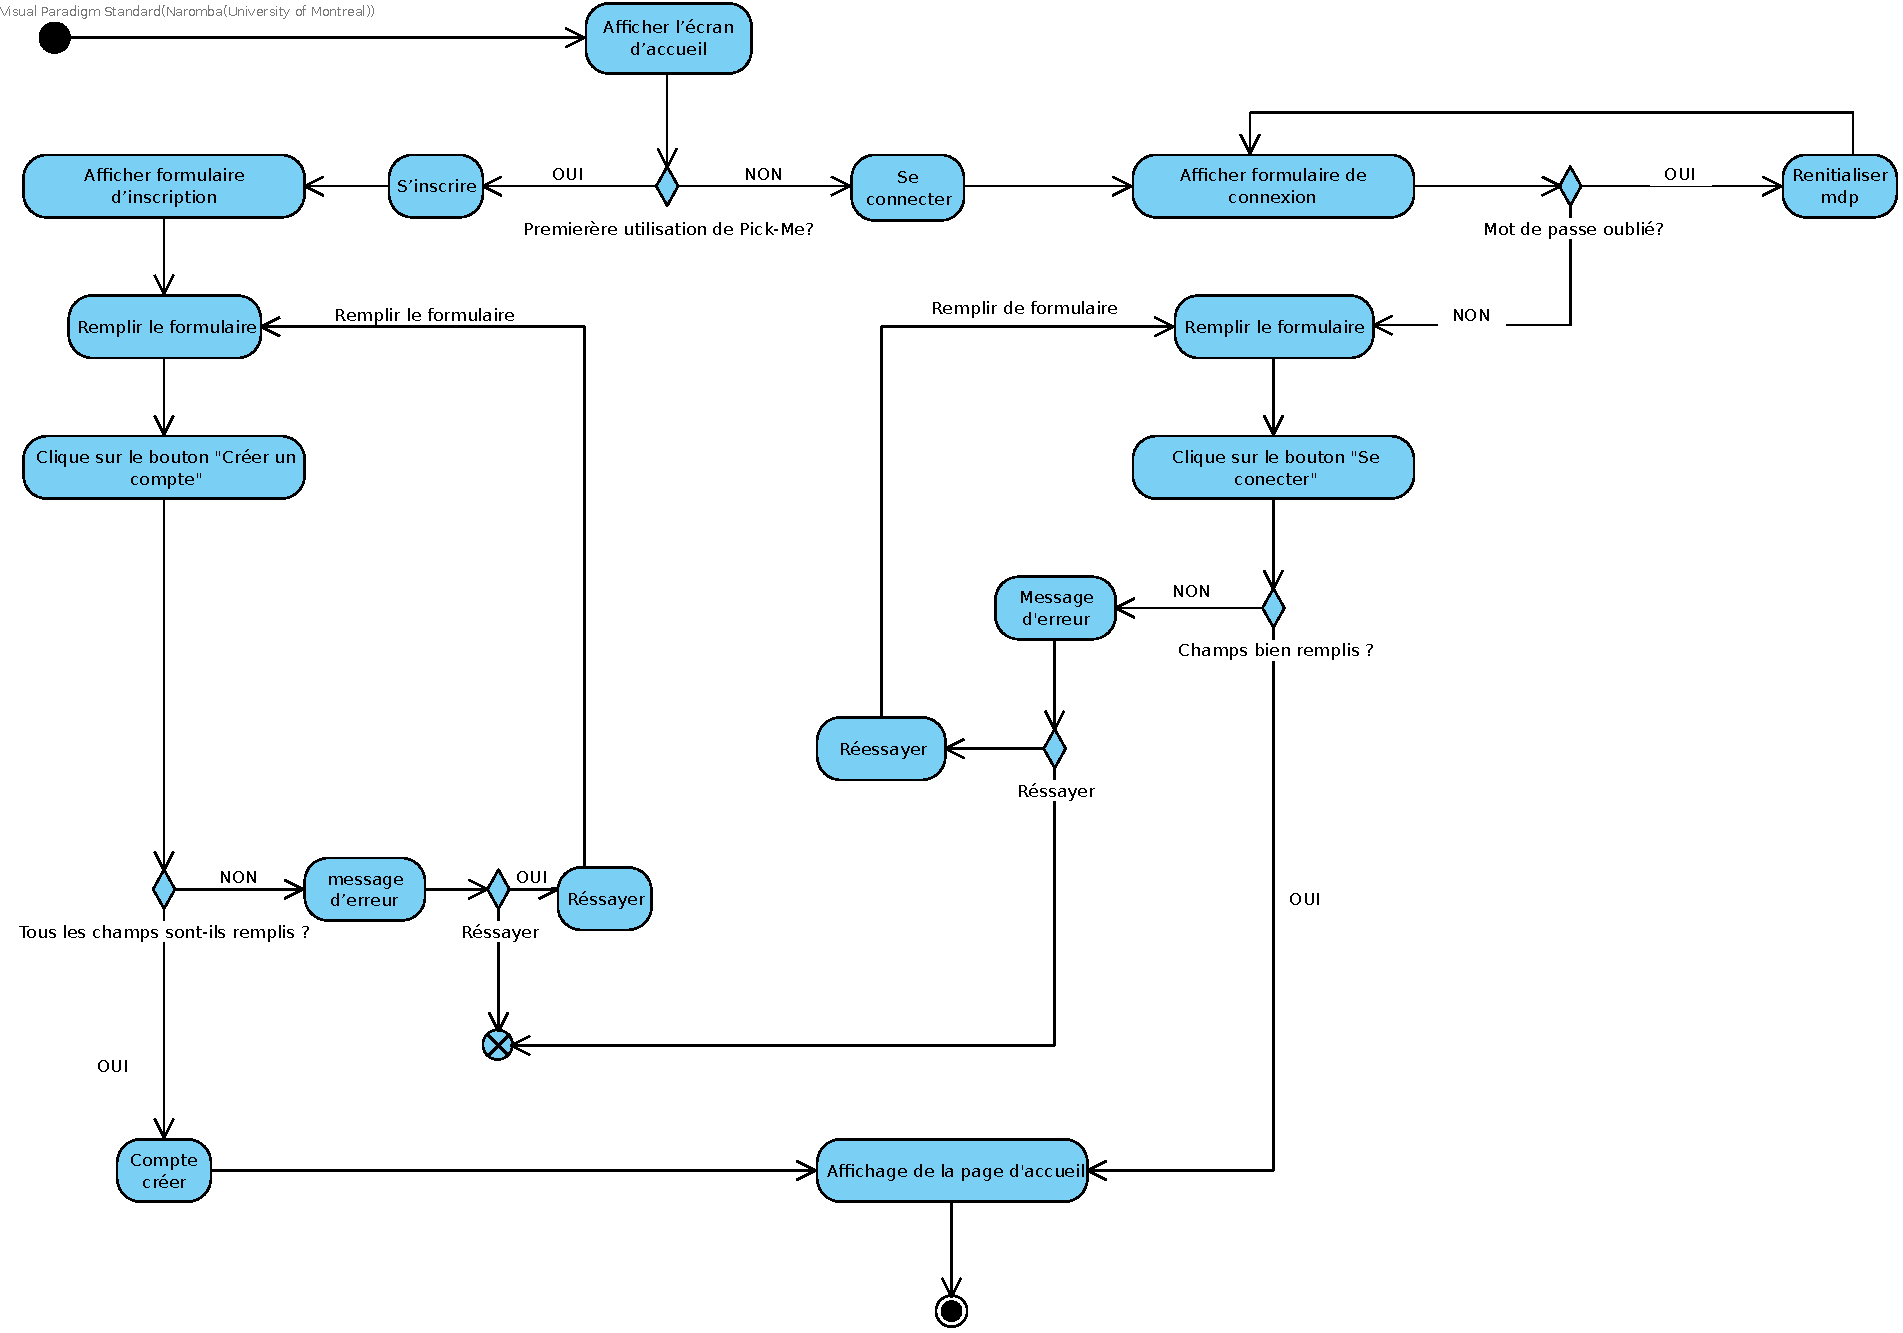
\includegraphics[width=0.9\linewidth]{attachments/Inscription_Connexion.pdf}
  \caption{Flux : Inscription et connexion}
\end{figure}

\subsubsection{Recherche et filtrage de parcs}

Ce diagramme montre le processus de recherche et de filtrage des parcs par l'utilisateur.

\begin{figure}[H]
  \centering
  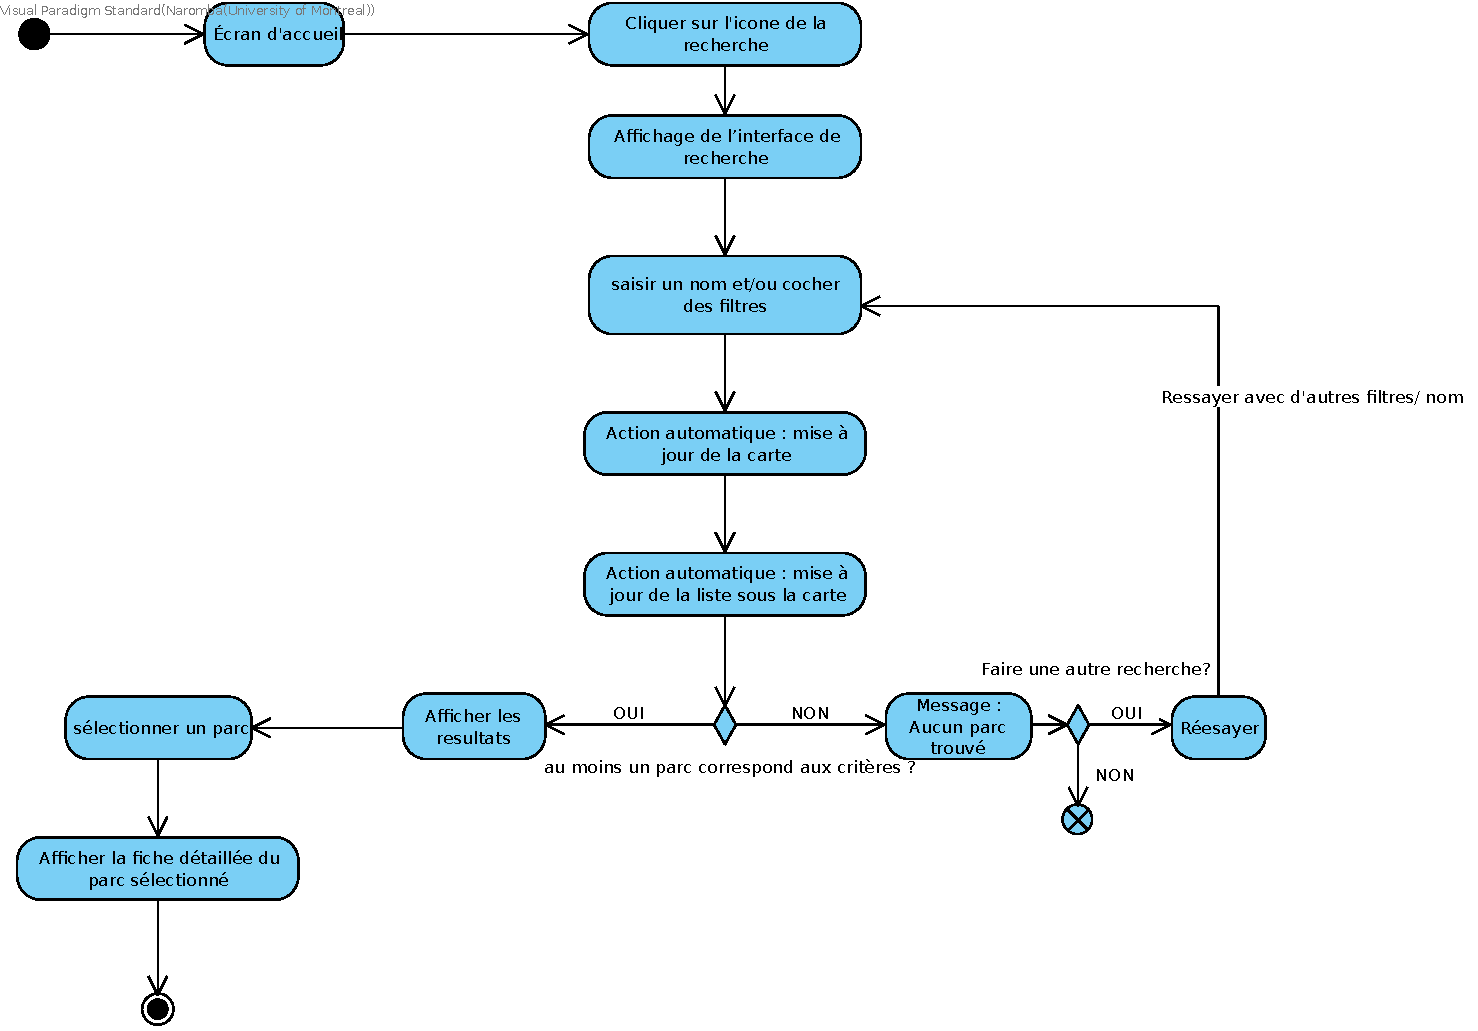
\includegraphics[width=0.9\linewidth]{attachments/Recherche_Filtrage_Parcs.pdf}
  \caption{Flux : Recherche et filtrage de parcs}
\end{figure}

\subsubsection{Réservation d'un emplacement}

Parcours utilisateur pour choisir un emplacement sur la carte du parc, sélectionner une date/heure puis confirmer la réservation.

\begin{figure}[H]
  \centering
  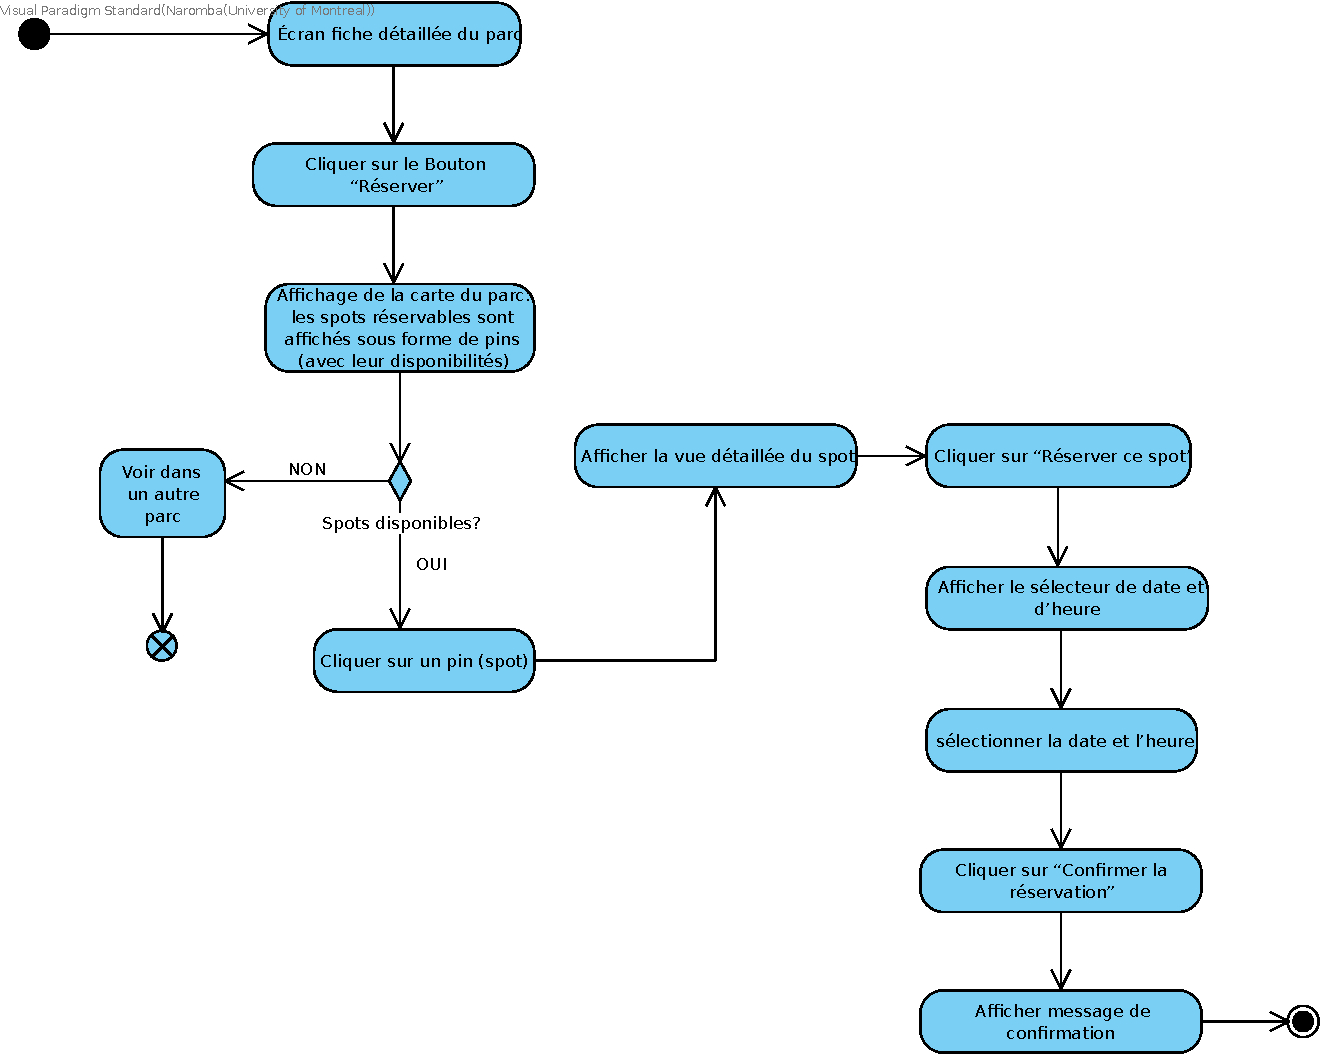
\includegraphics[width=0.9\linewidth]{attachments/Reservation_d_un_emplacement.pdf}
  \caption{Flux : Réservation d'un emplacement}
\end{figure}

\subsubsection{Réservation d'une activité}

Étapes pour sélectionner une activité dans la fiche du parc, choisir un créneau horaire et confirmer la réservation.

\begin{figure}[H]
  \centering
  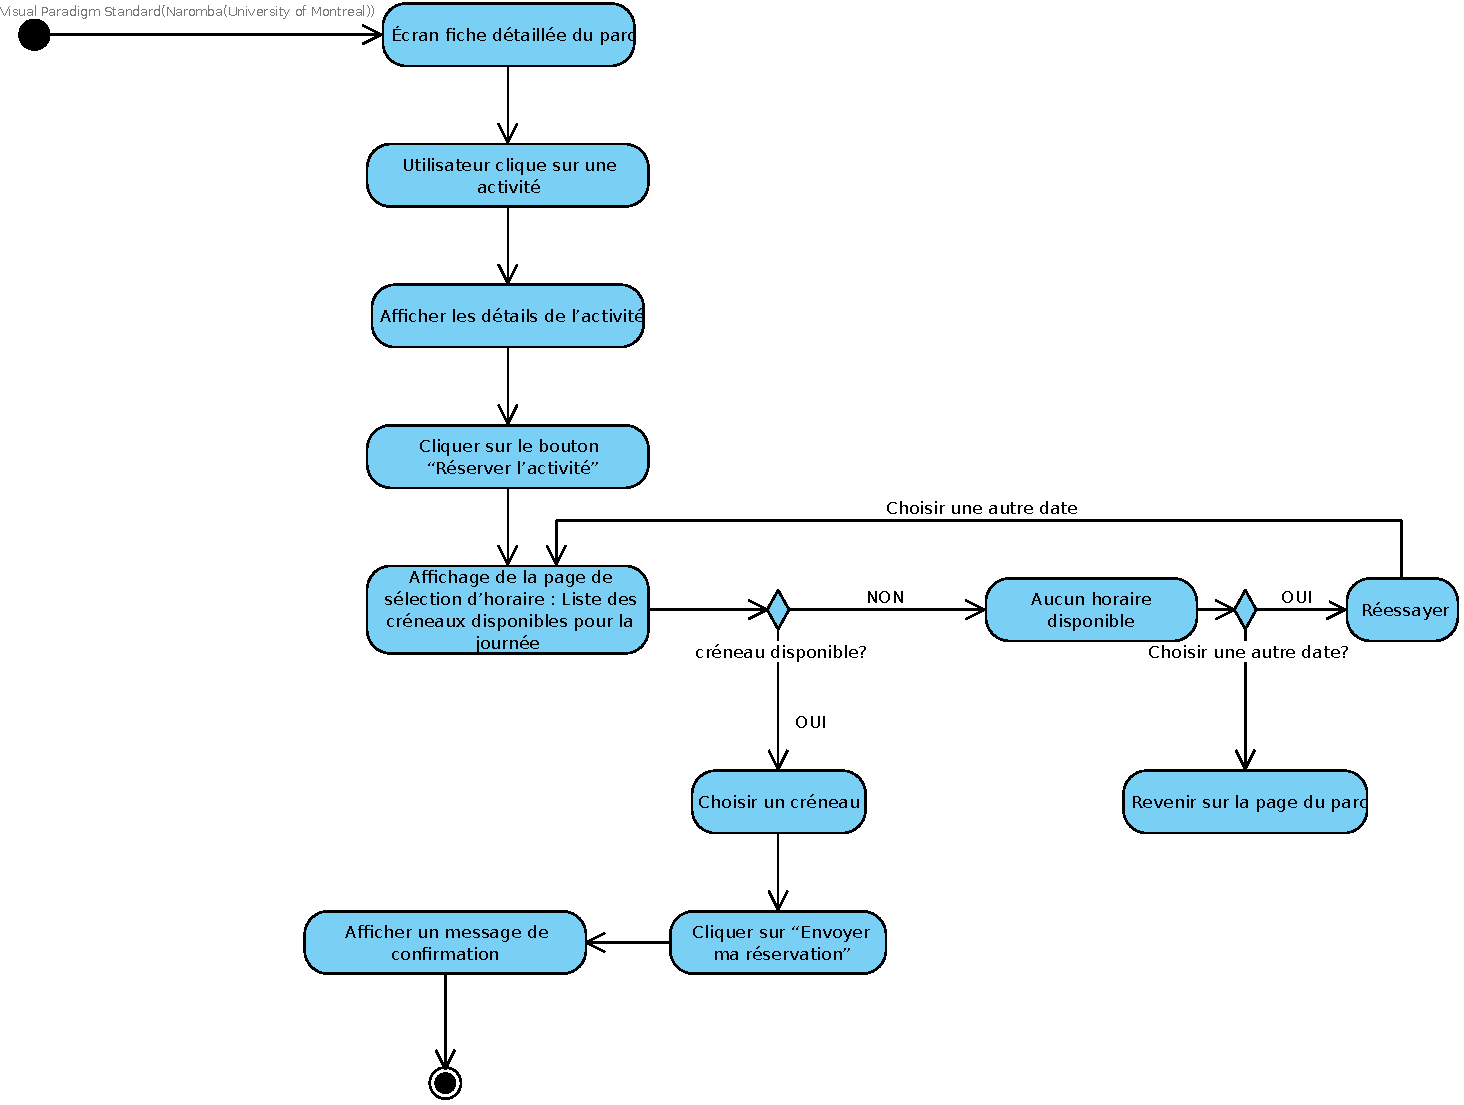
\includegraphics[width=0.9\linewidth]{attachments/Reservation_Activite.pdf}
  \caption{Flux : Réservation d'une activité}
\end{figure}

\subsubsection{Ajout ou retrait d'un favori}

Deux cas sont couverts : retirer un parc des favoris depuis la fiche du parc ou depuis la page des favoris.

\begin{figure}[H]
  \centering
  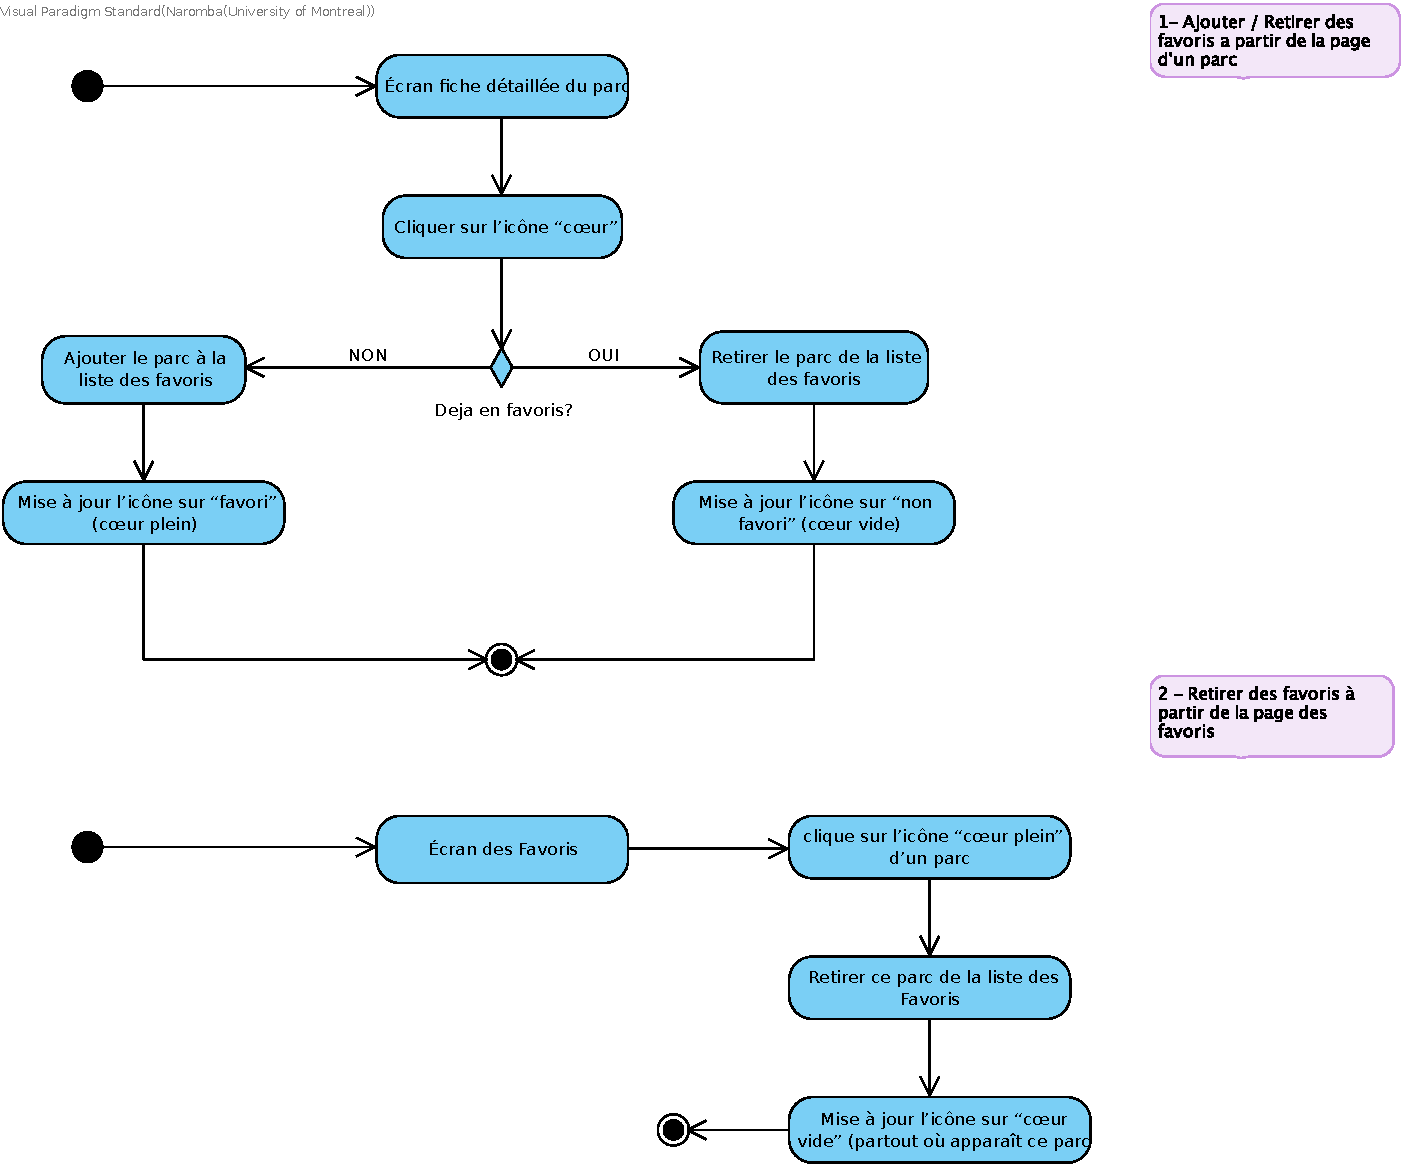
\includegraphics[width=0.9\linewidth]{attachments/Ajout_retrait_d_un_favori.pdf}
  \caption{Flux : Ajout / retrait d'un favori}
\end{figure}

\subsubsection{Ajout d'un avis}

L'utilisateur descend jusqu'à la section « Avis », saisit un commentaire, ajoute éventuellement une image, puis envoie son avis.

\begin{figure}[H]
  \centering
  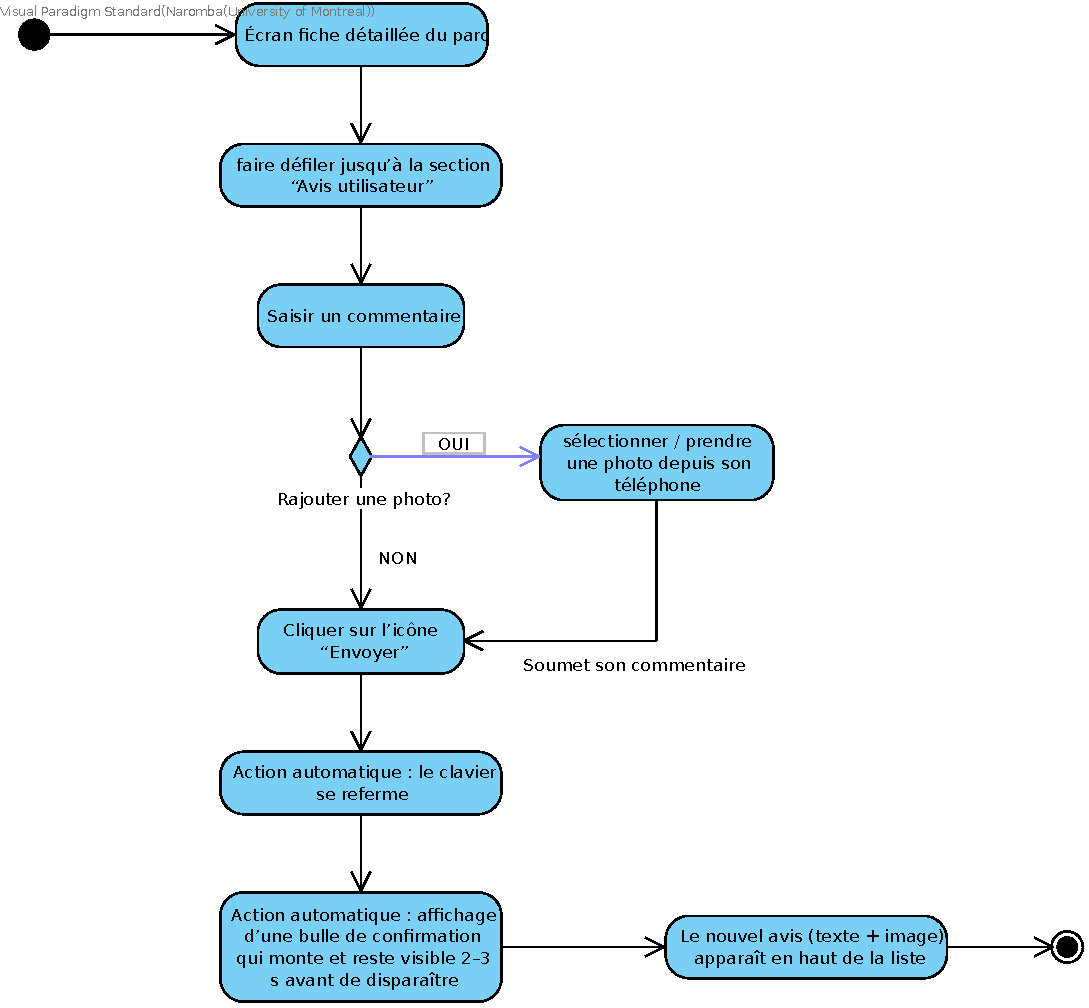
\includegraphics[width=0.9\linewidth]{attachments/Ajouter_un_avis_spot.pdf}
  \caption{Flux : Ajout d'un avis}
\end{figure}

\subsubsection{Sondage post-visite}

Après la visite, l'utilisateur reçoit une notification « Would you Pick-Me again ? », sélectionne des badges et peut laisser un commentaire.

\begin{figure}[H]
  \centering
  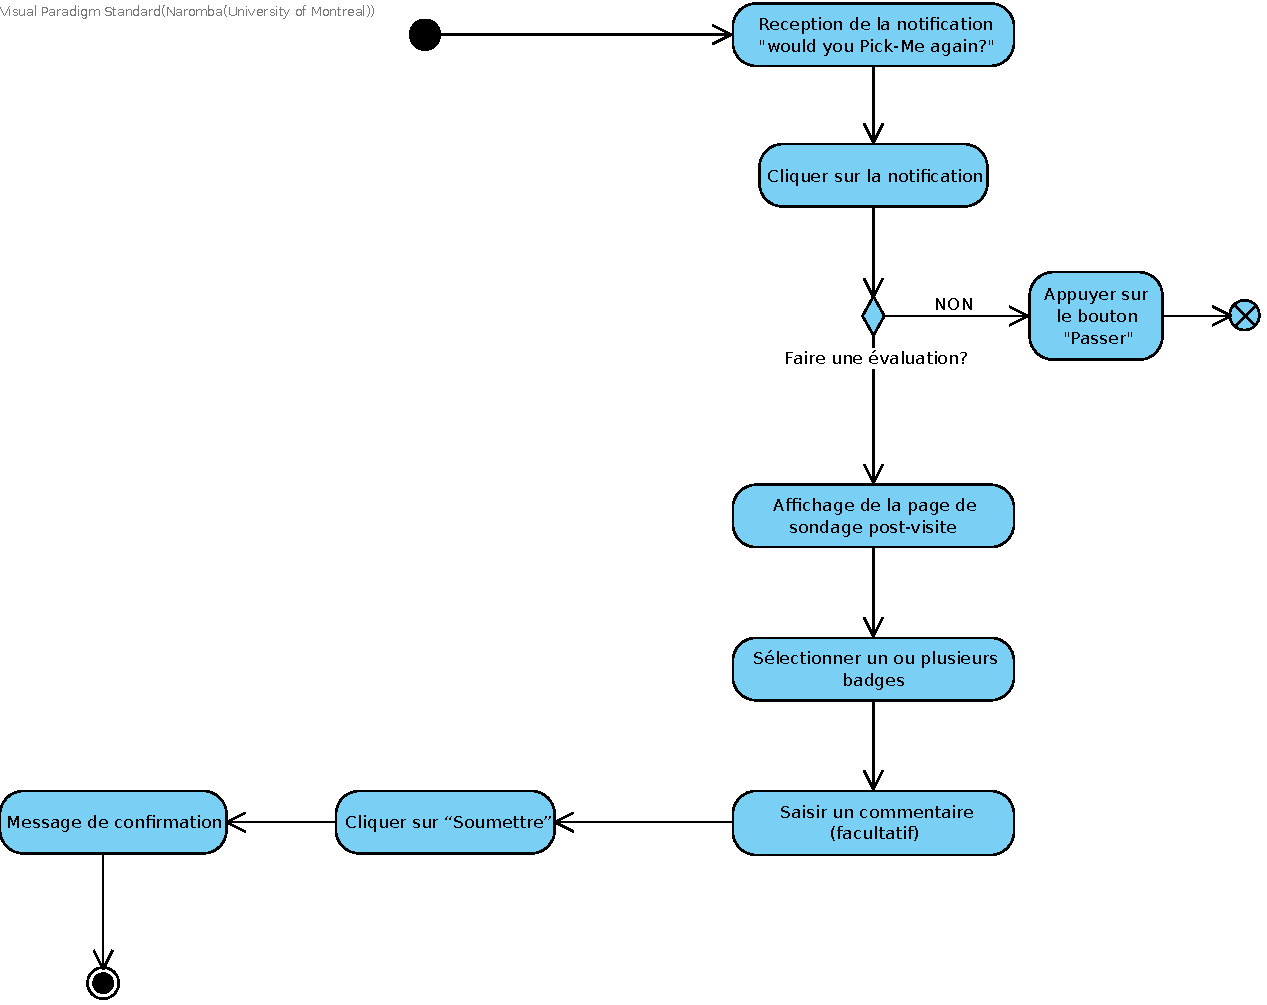
\includegraphics[width=0.9\linewidth]{attachments/Sondage_post_visite.pdf}
  \caption{Flux : Sondage post-visite}
\end{figure}

\subsection{Prototypes et maquettes}

Le design de l'application a été pensé pour offrir une expérience intuitive, visuelle et cohérente sur mobile. La maquette interactive a été conçue avec Figma.

\vspace{0.5em}
\noindent\textbf{Lien Figma :} \url{https://www.figma.com/design/kP7QEAejfvUB2yia4cleau/Pique-me?node-id=0-1}



\clearpage
% =========================================================
% 4. IMPLÉMENTATION ET RÉALISATION TECHNIQUE
% =========================================================
\section{Implémentation et réalisation technique}

Cette section décrit le fonctionnement réel de l’application côté mobile (écrans, navigation, données, interactions). Elle complète la section~3 (conception). À ce stade, nous n’utilisons plus de backend Node/Express en production : l’application accède directement au service de données (authentification, profils, favoris, réservations, avis) avec synchronisation en temps réel.

%----------------------------------------------------------
\subsection{Front-end uniquement : source de vérité et synchro}

\begin{itemize}
  \item \textbf{Données} : comptes, préférences, favoris, parcs (avec centroïde et geohash), avis et réservations sont stockés côté service de données et lus/écrits directement depuis l’app.
  \item \textbf{Temps réel} : les écrans s’abonnent aux collections/documents pertinents; toute mise à jour (ex.: ajout d’un favori) est répercutée instantanément dans l’UI, sans rechargement manuel.
  \item \textbf{Sécurité} : règles d’accès par utilisateur (lecture/écriture sur son profil, création d’avis, réservation atomique pour éviter les collisions).
\end{itemize}

%----------------------------------------------------------
\subsection{Recherche + Carte }

\begin{itemize}
  \item \textbf{Ouverture} : demande de permission de localisation, centrage initial sur l’utilisateur, définition d’une fenêtre (viewport) adaptée à l’écran.
  \item \textbf{Chargement progressif} : les parcs visibles dans la fenêtre courante sont affichés en premier pour donner une première réponse rapide; le reste est chargé en arrière-plan.
  \item \textbf{Filtrage local} : la barre de recherche (texte sans accents) et les étiquettes (ex.: aire de jeu, pique-nique) filtrent \emph{uniquement} ce qui est à l’écran, pour préserver fluidité et lisibilité.
  \item \textbf{Liste liée à la carte} : un panneau coulissant présente la liste synchronisée des mêmes résultats; taper un élément ouvre sa fiche.
\end{itemize}

%----------------------------------------------------------
\subsection{Fiche parc : actions clés}

\begin{itemize}
  \item \textbf{Contenu} : galerie d’images, équipements/activités dérivés des installations, note visuelle, bouton \og Réserver \fg.
  \item \textbf{Favori} : l’icône cœur bascule l’état et l’enregistre immédiatement; l’information se répercute sur la liste et la carte sans délai.
  \item \textbf{Avis} : saisie simple (texte + photo optionnelle) et badges thématiques. Les agrégations (seuils bronze/argent/or) sont reflétées sur la fiche.
\end{itemize}

%----------------------------------------------------------
\subsection{Réservation : flux et garanties}

\begin{itemize}
  \item \textbf{Étapes} : choix d’un emplacement sur la carte du parc, puis sélection d’un créneau horaire.
  \item \textbf{Validation} : enregistrement immédiat et retour visuel; rappels avant l’heure prévue; annulation automatique en cas de non-confirmation après le début.
  \item \textbf{Concurrence} : écriture atomique pour empêcher deux réservations sur le même créneau; message clair si déjà pris.
\end{itemize}

%----------------------------------------------------------
\subsection{Favoris et profil}

\begin{itemize}
  \item \textbf{Favoris} : page dédiée avec les parcs enregistrés; toute action (ajout/retrait) est visible sur tous les écrans grâce à la synchro temps réel.
  \item \textbf{Profil} : mise à jour du nom, du mot de passe et des préférences (tags). Les préférences nourrissent les recommandations d’accueil et influencent la recherche.
\end{itemize}

%----------------------------------------------------------
\subsection{Navigation (Expo Router) }

\begin{itemize}
  \item \textbf{Paramètres} : ouverture d’une fiche avec l’identifiant du parc; passage des coordonnées/infos utiles au flux de réservation; retour natif pris en charge.
  \item \textbf{UX mobile} : transitions natives, panneau coulissant pour la liste, et icône cœur en surimpression dans les galeries.
\end{itemize}

%----------------------------------------------------------
\subsection{Notes d’implémentation côté code }

\begin{itemize}
  \item \textbf{Composants réutilisables} : cartes de parc, carrousel d’images, badges/étoiles, champ d’avis. Les propriétés restent simples pour limiter les effets de bord.
  \item \textbf{État minimal global} : utilisateur, préférences et favoris sont partagés; le reste (scroll, pagination, sélection locale) reste proche des écrans.
  \item \textbf{Performance} : limitation des marqueurs à la zone visible, chargement progressif, pagination visuelle des images; filtrage local pour éviter des requêtes inutiles.
  \item \textbf{Robustesse UX} : gestion explicite des permissions (localisation, galerie) et messages d’erreur compréhensibles en cas de souci réseau.
\end{itemize}




%----------------------------------------------------------
\subsection{Difficultés résolues}

\begin{itemize}
  \item \textbf{Fusion de données publiques :} les informations sur les parcs étaient réparties dans plusieurs fichiers (localisation, équipements et activités). Nous avons dû croiser et nettoyer ces données pour n'avoir qu'un seul format clair à utiliser dans l'application.
  
  \item \textbf{Interrogation des API trop lente :} certaines sources prenaient jusqu'à deux minutes pour répondre. Nous avons donc décidé d'extraire leurs données à l'avance et de les importer une fois pour toutes dans Firebase.

  \item \textbf{Problèmes de réservation en double :} pour éviter que deux utilisateurs réservent le même créneau, nous avons utilisé une vérification automatique côté base de données. Si le créneau est déjà pris, un message d'erreur clair s'affiche.

  \item \textbf{Affichage pas toujours à jour :} au début, il arrivait que les favoris ou les avis ne se mettent pas à jour tout de suite. Nous avons corrigé cela en connectant directement les composants d'affichage à Firebase. Ainsi, tout changement est visible en temps réel, sans avoir besoin de recharger l'écran.
\end{itemize}

%----------------------------------------------------------


\clearpage
% =========================================================
% 5. ÉVALUATION
% =========================================================
\section{Évaluation}
\subsection{Tests unitaires et fonctionnels}
\subsection{Évaluation de performance}
\subsection{Évaluation d'utilisabilité}
\subsection{Comparaison avec les objectifs initiaux}


\clearpage
% =========================================================
% 6. DISCUSSION CRITIQUE
% =========================================================
\section{Discussion critique}

La version actuelle de \textit{Pique-Me} atteint son objectif premier :
offrir, sur mobile, un moyen simple de découvrir les parcs de Montréal,
de réserver un emplacement et de partager son expérience. 

\medskip\noindent
\textbf{Analyse critique.}  
Le choix d'un socle « Firebase » a apporté un réel confort : pas de
serveur à maintenir, sécurité intégrée, mises à jour en temps réel
gratuites. En revanche, cette dépendance impose certaines limites :
logique métier cantonnée aux règles Firestore, format de requête parfois
rigide, et difficulté à exécuter des traitements lourds côté serveur. La structure en mini-composants
React facilite grandement la maintenance ; toutefois, elle augmente
aussi le nombre de fichiers à gérer et peut alourdir la prise en main
pour un nouveau développeur.

\medskip\noindent
\textbf{Problèmes rencontrés et solutions mises en place.}
\begin{itemize}
  \item \emph{Données éparpillées :} les informations officielles
        provenaient de trois sources lentes et incomplètes. Nous avons
        donc écrit un script d'import qui fusionne et nettoie ces
        fichiers, puis les stocke dans une seule collection
        \texttt{parks}. Temps de réponse côté appli : divisé par dix.
  \item \emph{API cartographique saturée :} afficher 500 parcs à la fois
        rendait la carte illisible. Nous limitons maintenant les
        marqueurs au rayon de 2 km ; les autres parcs se chargent au
        besoin quand on dézoome.
  \item \emph{Réservations en double :} deux utilisateurs pouvaient,
        durant les premiers tests, choisir le même créneau. Désormais,
        une transaction Firestore bloque la seconde requête et renvoie
        un message explicite.
  \item \emph{Synchronisation des favoris :} il arrivait qu'un cœur
        reste allumé sur un écran mais pas sur l'autre. Tous les
        composants « carte de parc » écoutent maintenant directement
        les changements Firebase ; l'affichage est harmonisé sans
        rechargement manuel.
\end{itemize}

\medskip\noindent
\textbf{Ce qui pourrait être amélioré avec plus de temps ou de moyens.}
\begin{itemize}
  \item \emph{Suggestions communautaires :} permettre aux utilisateurs
        d'ajouter eux-mêmes de nouveaux parcs ou équipements encore non
        répertoriés, photos à l'appui.
  \item \emph{Recommandations plus fines :} analyser les avis pour
        proposer des parcs en fonction du moment de la journée, de la
        météo ou d'événements spéciaux.
  \item \emph{Plateformes supplémentaires :} décliner l'application en
        version tablette et web pour toucher un public plus large :
        familles planifiant leurs sorties depuis un salon ou écoles
        préparant des activités extérieures.
  \item \emph{Fonctions hors ligne étendues :} permettre le
        téléchargement d'un arrondissement complet afin d'utiliser la
        recherche cartographique sans réseau du tout.
  \item \emph{Interface adaptable :} proposer un mode « gaucher »
        (boutons principaux inversés) et des options d'accessibilité
        supplémentaires (taille de police, contraste renforcé).
  \item \emph{Multilingue :} offrir l'application en français et en
        anglais (et d'autres langues à terme) afin d'être inclusive
        pour les résidents et touristes.
\end{itemize}


\medskip\noindent

\clearpage
% =========================================================
% 7. CONCLUSION
% =========================================================
\section{Conclusion}

Le projet \textit{Pique-Me} visait à simplifier l'expérience des citoyens dans les parcs urbains : trouver le bon lieu, réserver un espace et partager un avis. En quatre mois, nous avons livré une application mobile fluide, capable d'afficher les parcs pertinents en quelques secondes et de synchroniser réservations ou favoris en temps réel. 

\medskip\noindent
\textbf{Leçons tirées.}  
Nous avons mesuré la force et les limites d'une solution entièrement basée sur Firebase : elle accélère la mise en œuvre et la synchronisation, mais impose un format de requête strict. L'approche « mini-composants » sous React Native s'est révélée payante : chaque pièce est réutilisable et testable isolément, limitant les régressions. Enfin, fusionner plusieurs jeux de données publics nous a appris qu'un nettoyage rigoureux avant importation est indispensable pour garantir une source unique et fiable.

\medskip\noindent
\textbf{Pistes d'amélioration.}  
\begin{itemize}
  \item \emph{Fonctions communautaires élargies :} permettre aux usagers de proposer de nouveaux parcs ou équipements, photos à l'appui.
  \item \emph{Recommandations personnalisées :} intégrer la météo, l'heure de la journée et les avis pour suggérer le parc idéal à chaque instant.
  \item \emph{Accessibilité renforcée :} mode gaucher, tailles de texte adaptatives, synthèse vocale pour la navigation.
  \item \emph{Version web et tablette :} offrir la même expérience sur grand écran, utile aux familles et aux écoles.
  \item \emph{Mode hors-ligne complet :} téléchargement d'un arrondissement pour une consultation sans réseau, puis synchronisation différée.
\end{itemize}

\medskip\noindent
En définitive, \textit{Pique-Me} prouve qu'une architecture simple et modulaire peut rendre un service concret et apprécié. Avec ces améliorations, nous pourrons \textbf{étendre la couverture et faire de \textit{Pique-Me} l'outil de référence des sorties dans les parcs montréalais}.


\clearpage
% =========================================================
% 8. REMERCIEMENTS (facultatif)
% =========================================================
\section*{Remerciements}

Nous souhaitons exprimer notre gratitude envers nos collègues \textbf{Marc Oliver Jean paul} et \textbf{Lallia Diakité}, avec qui nous avons partagé le développement de ce projet dans le cadre du cours \textit{Interface personne-machine}. Leur collaboration, leur écoute et leur motivation ont grandement contribué à la réussite de ce travail.

Nous remercions également \textbf{M. Louis-Édouard Lafontant}, notre enseignant, pour son accompagnement tout au long de la session. Présent à chaque étape, il a su répondre à toutes nos questions avec rigueur et bienveillance, parfois dans le cadre de discussions (très) longues mais toujours constructives. Il n'a pas hésité à nous faire retravailler plusieurs éléments pour atteindre un meilleur rendu.

Enfin, nous tenons à saluer \textbf{notre propre engagement} : malgré une session intense, nous avons su rester investis, rigoureux et persévérants, jusqu'à la finalisation de ce projet.


\clearpage
% =========================================================
% 9. RÉFÉRENCES
% =========================================================
\section*{Références}

\begin{itemize}

  \item Google. (2024). \textit{Documentation Firebase}. Disponible en ligne : \url{https://firebase.google.com/docs}

  \item Ville de Montréal. (2024). \textit{API publiques — données sur les parcs, équipements et activités}. \emph{(....)}.

  \item Meta. (2024). \textit{Documentation React Native}. Composants de base, navigation et gestion d'état. \emph{(....)}.

  \item OpenAI. (2025). \textit{Assistance à la rédaction et au débogage via ChatGPT}. \url{https://chat.openai.com}
\end{itemize}


\clearpage
% =========================================================
% 10. ANNEXES
% =========================================================
\appendix
\section{Annexes}

Capture d'écran des principales pages du prototype Figma:

\begin{figure}[h!]
  \centering
  \begin{minipage}[t]{0.45\linewidth}
    \vtop{
      \centering
      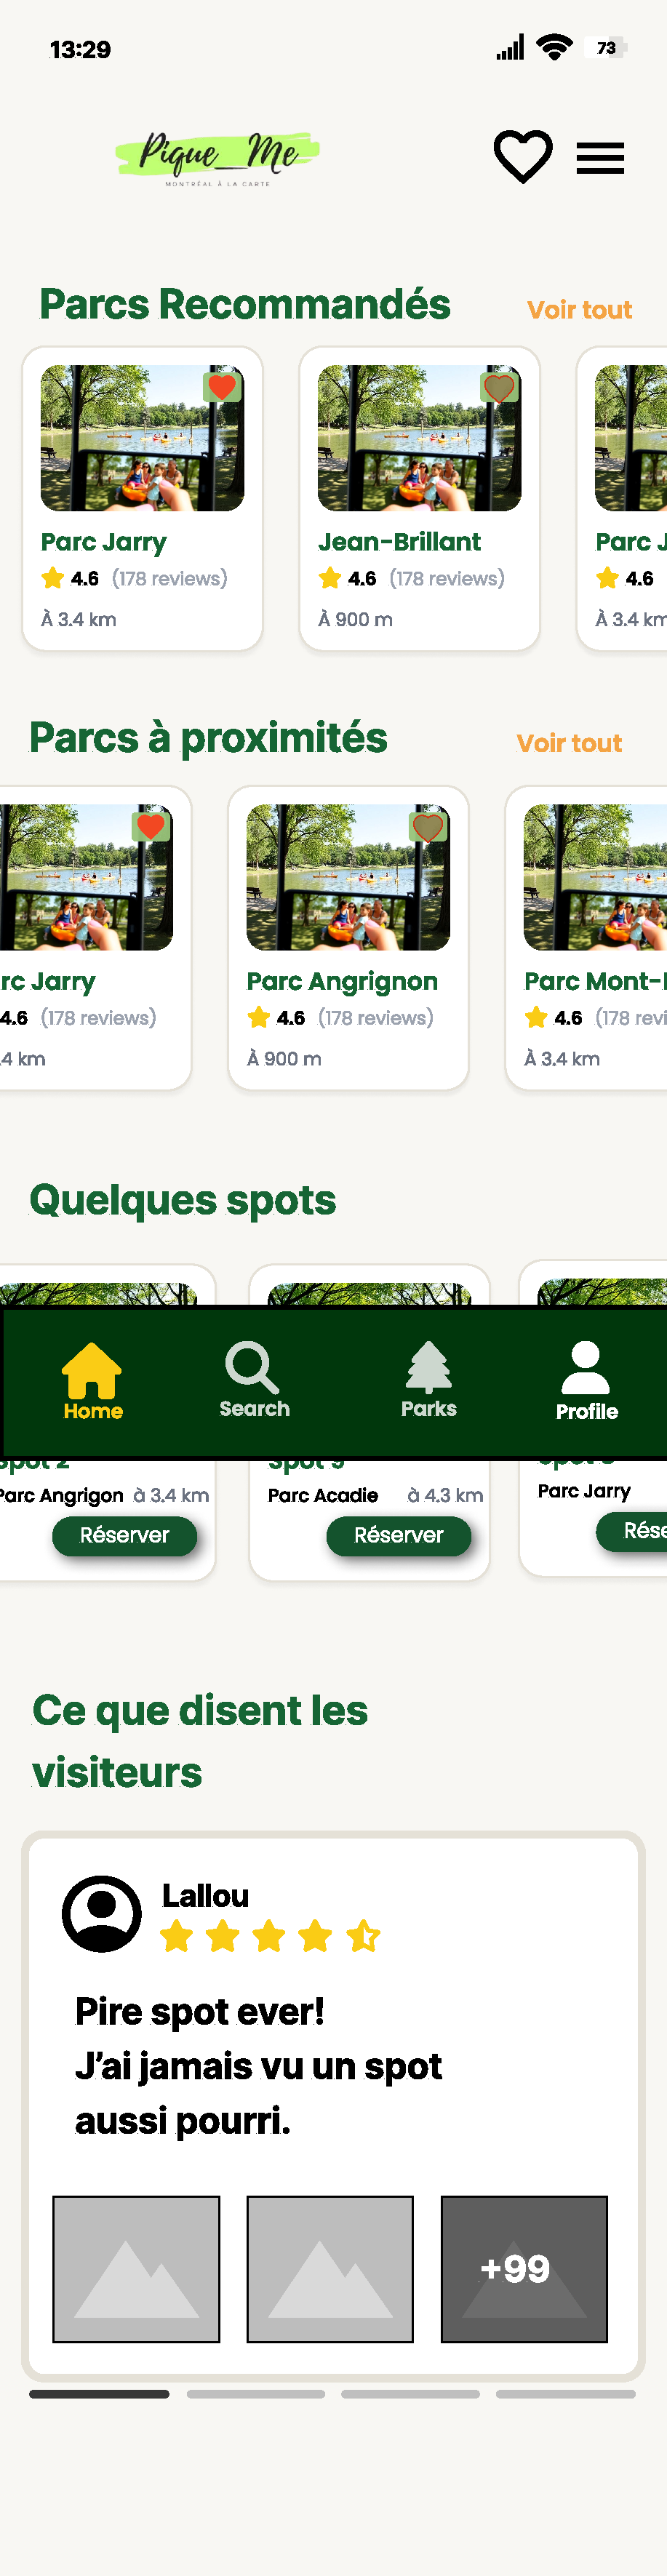
\includegraphics[height=3\linewidth]{attachments/HomeConnected.pdf}
      \caption{Page d'accueil.}
    }
  \end{minipage}
  \hfill
  \begin{minipage}[t]{0.45\linewidth}
    \vtop{
      \centering
      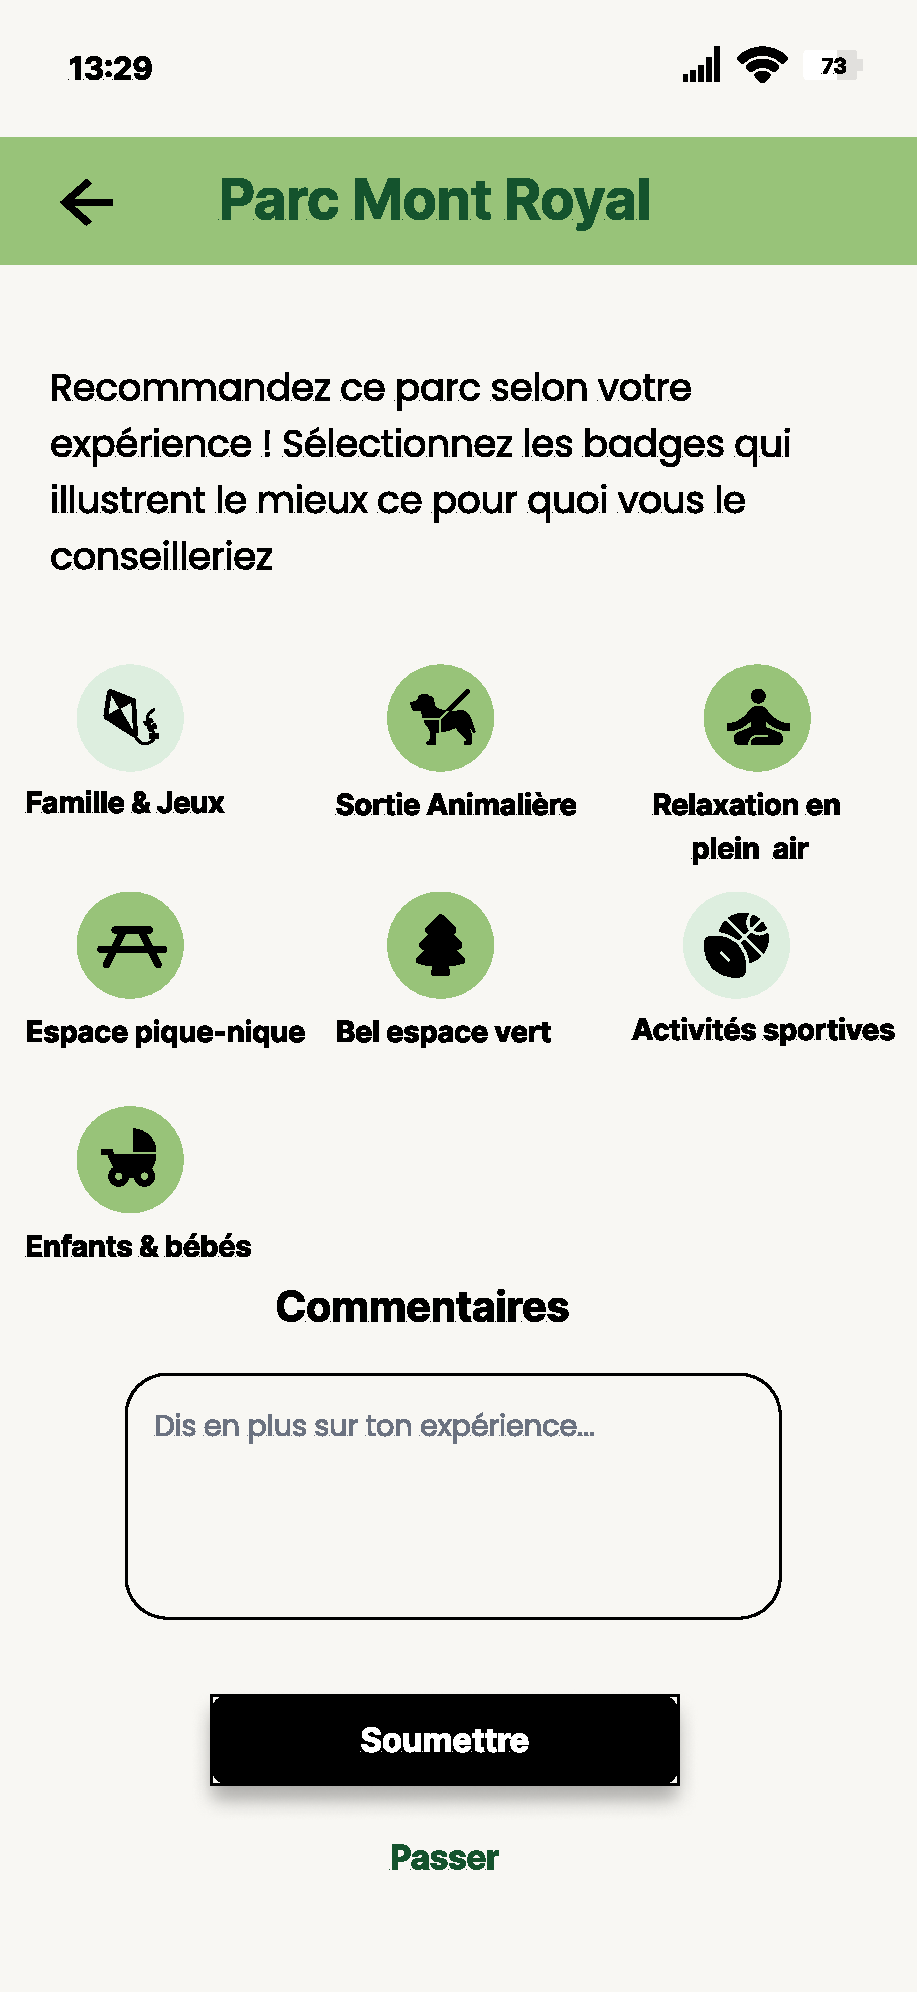
\includegraphics[width=\linewidth]{attachments/Evaluation1.pdf}
      \caption{Page d'évaluation.}
    }
  \end{minipage}
\end{figure}

\begin{figure}[h!]
  \centering
  \begin{minipage}[t]{0.45\linewidth}
    \vtop{
      \centering
      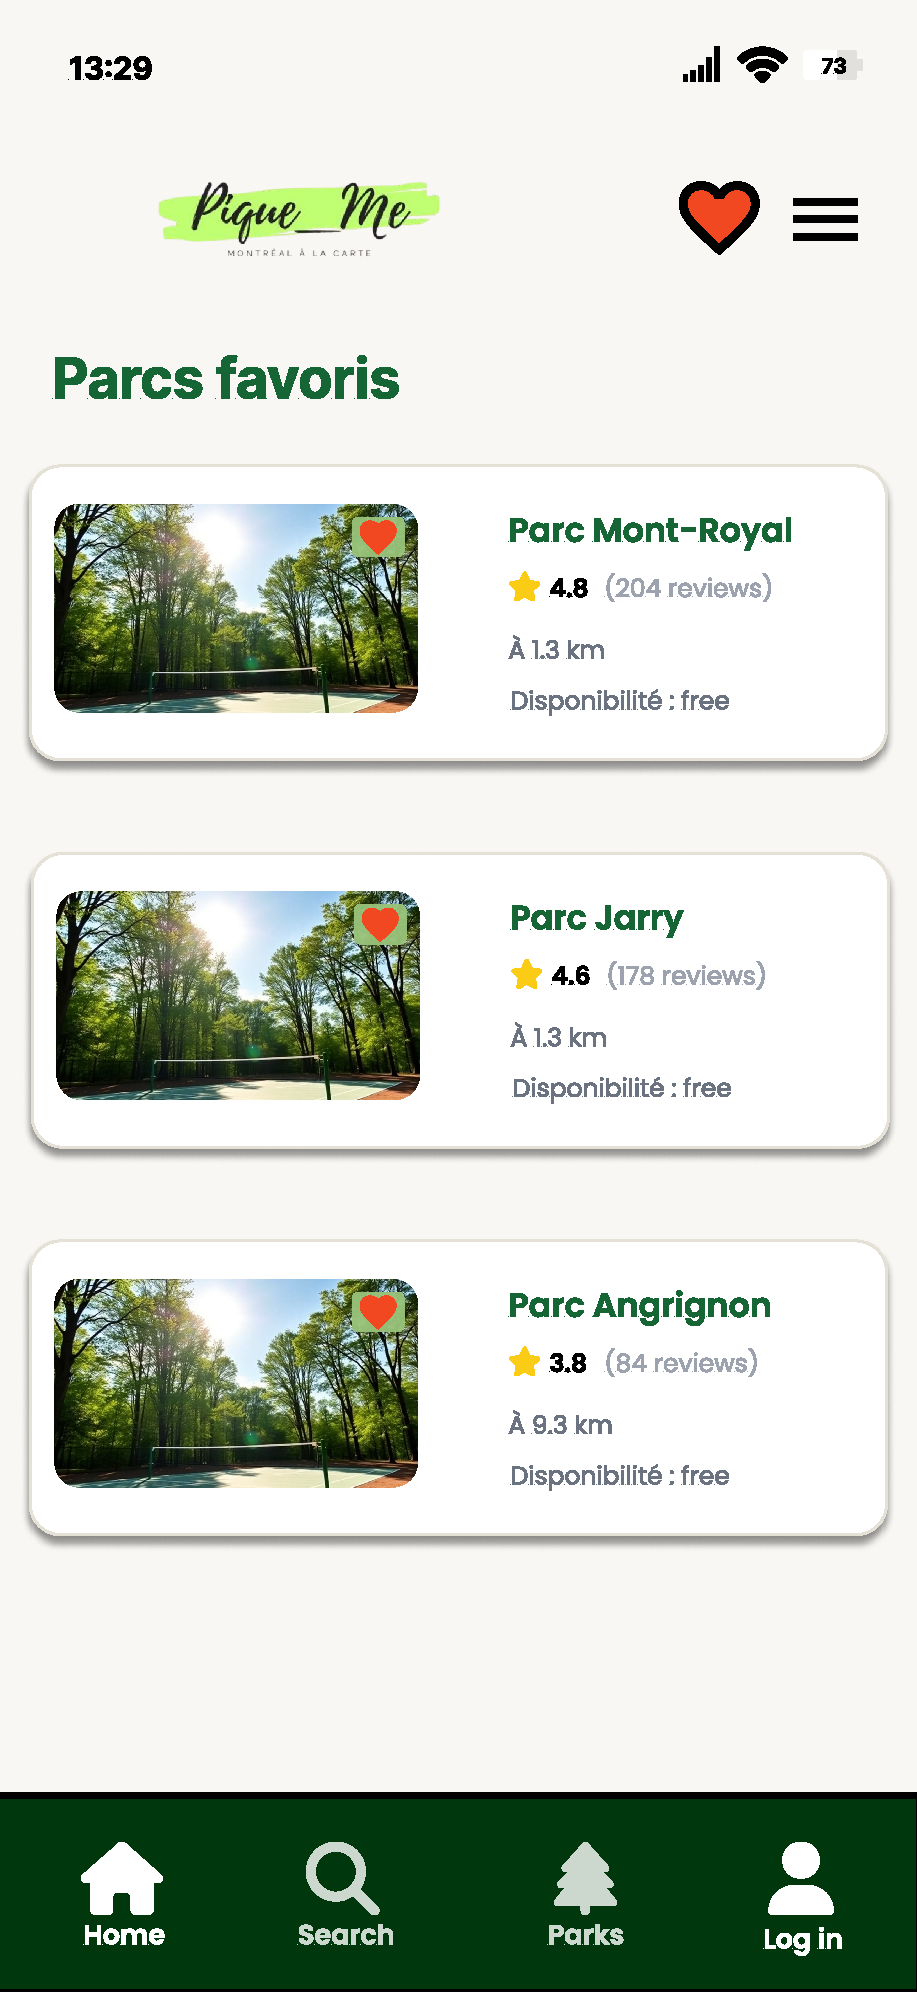
\includegraphics[width=\linewidth]{attachments/PageParcsFavori.pdf}
      \caption{Page des favoris.}
    }
  \end{minipage}
  \hfill
  \begin{minipage}[t]{0.45\linewidth}
    \vtop{
      \centering
      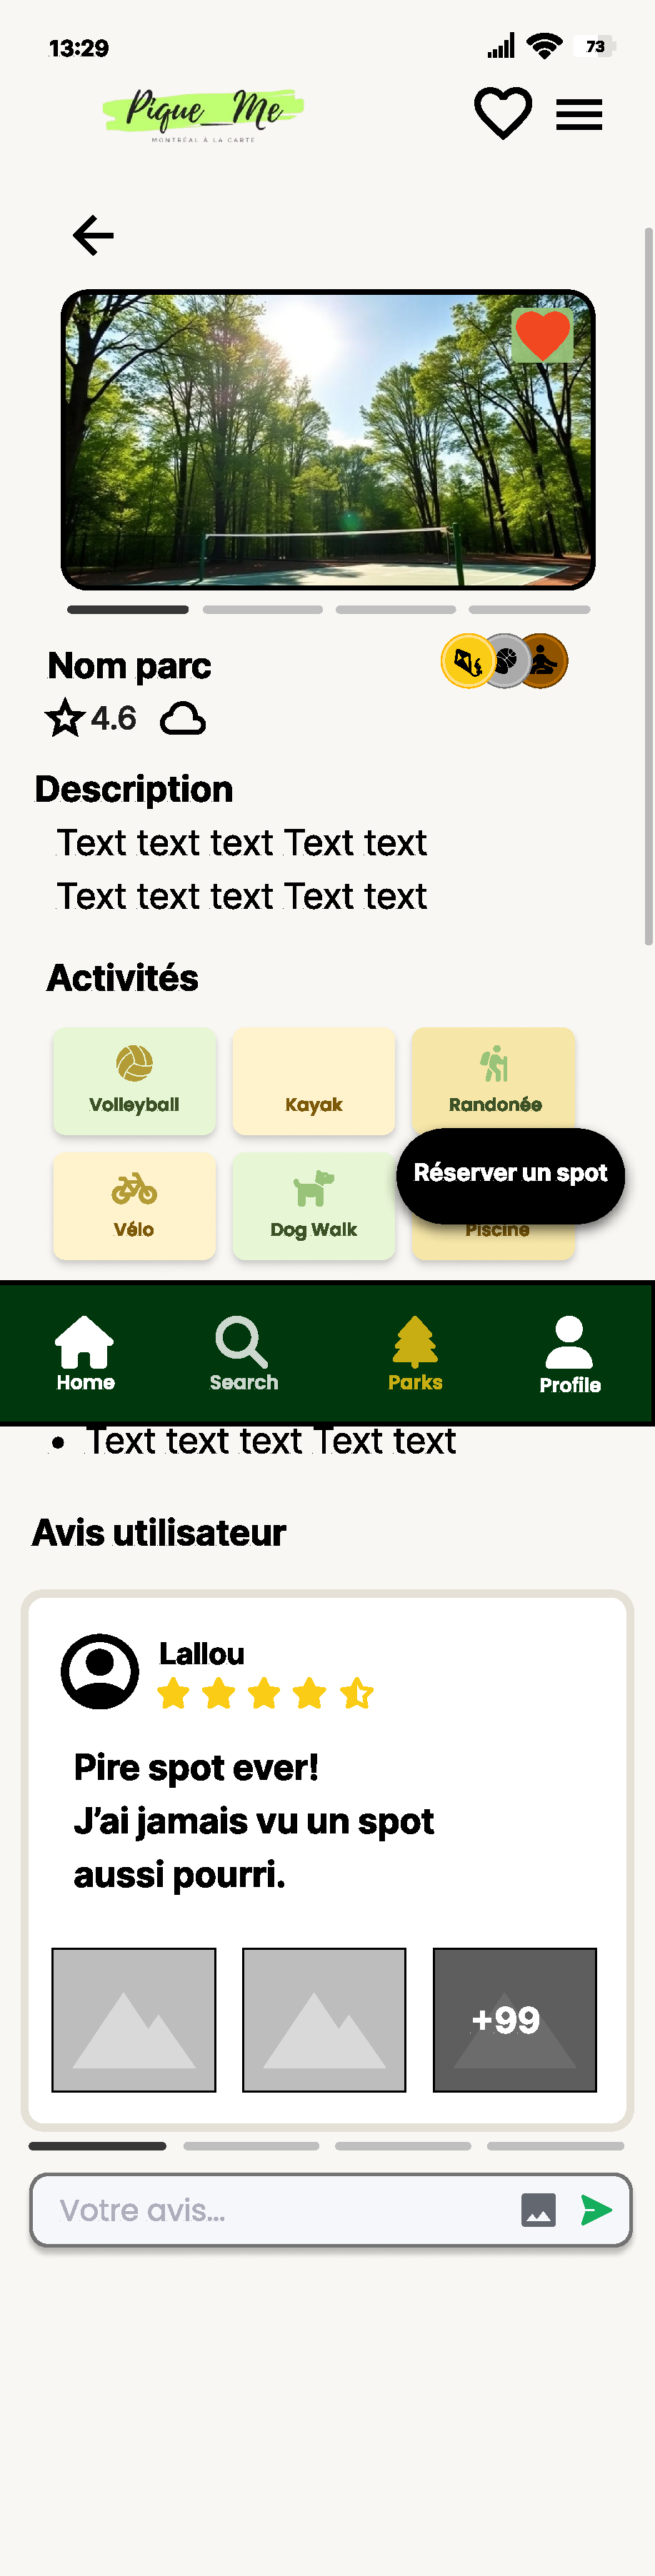
\includegraphics[height=3\linewidth]{attachments/pageParc.pdf}
      \caption{Page d'un parc.}
    }
  \end{minipage}
\end{figure}

\begin{figure}[h!]
  \centering
  \begin{minipage}[t]{0.45\linewidth}
    \vtop{
      \centering
      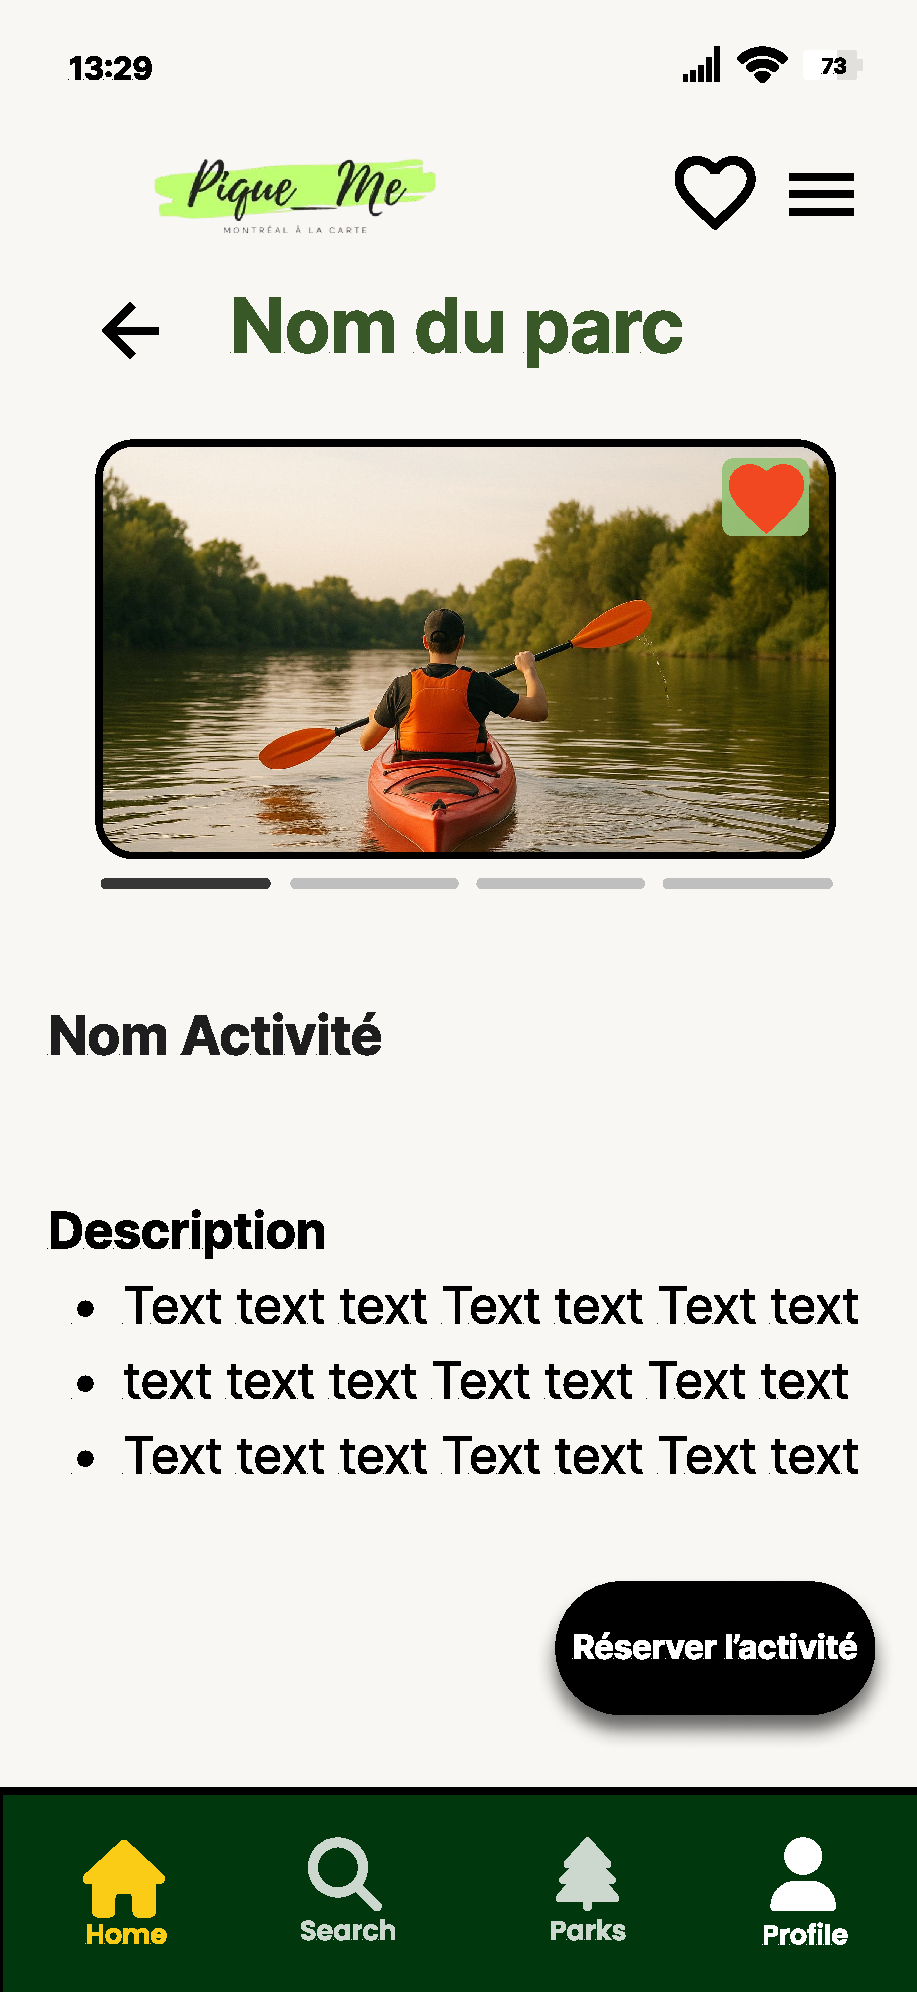
\includegraphics[width=\linewidth]{attachments/PageActivite.pdf}
      \caption{Page d'une activité si elle est réservable.}
    }
  \end{minipage}
  \hfill
  \begin{minipage}[t]{0.45\linewidth}
    \vtop{
      \centering
      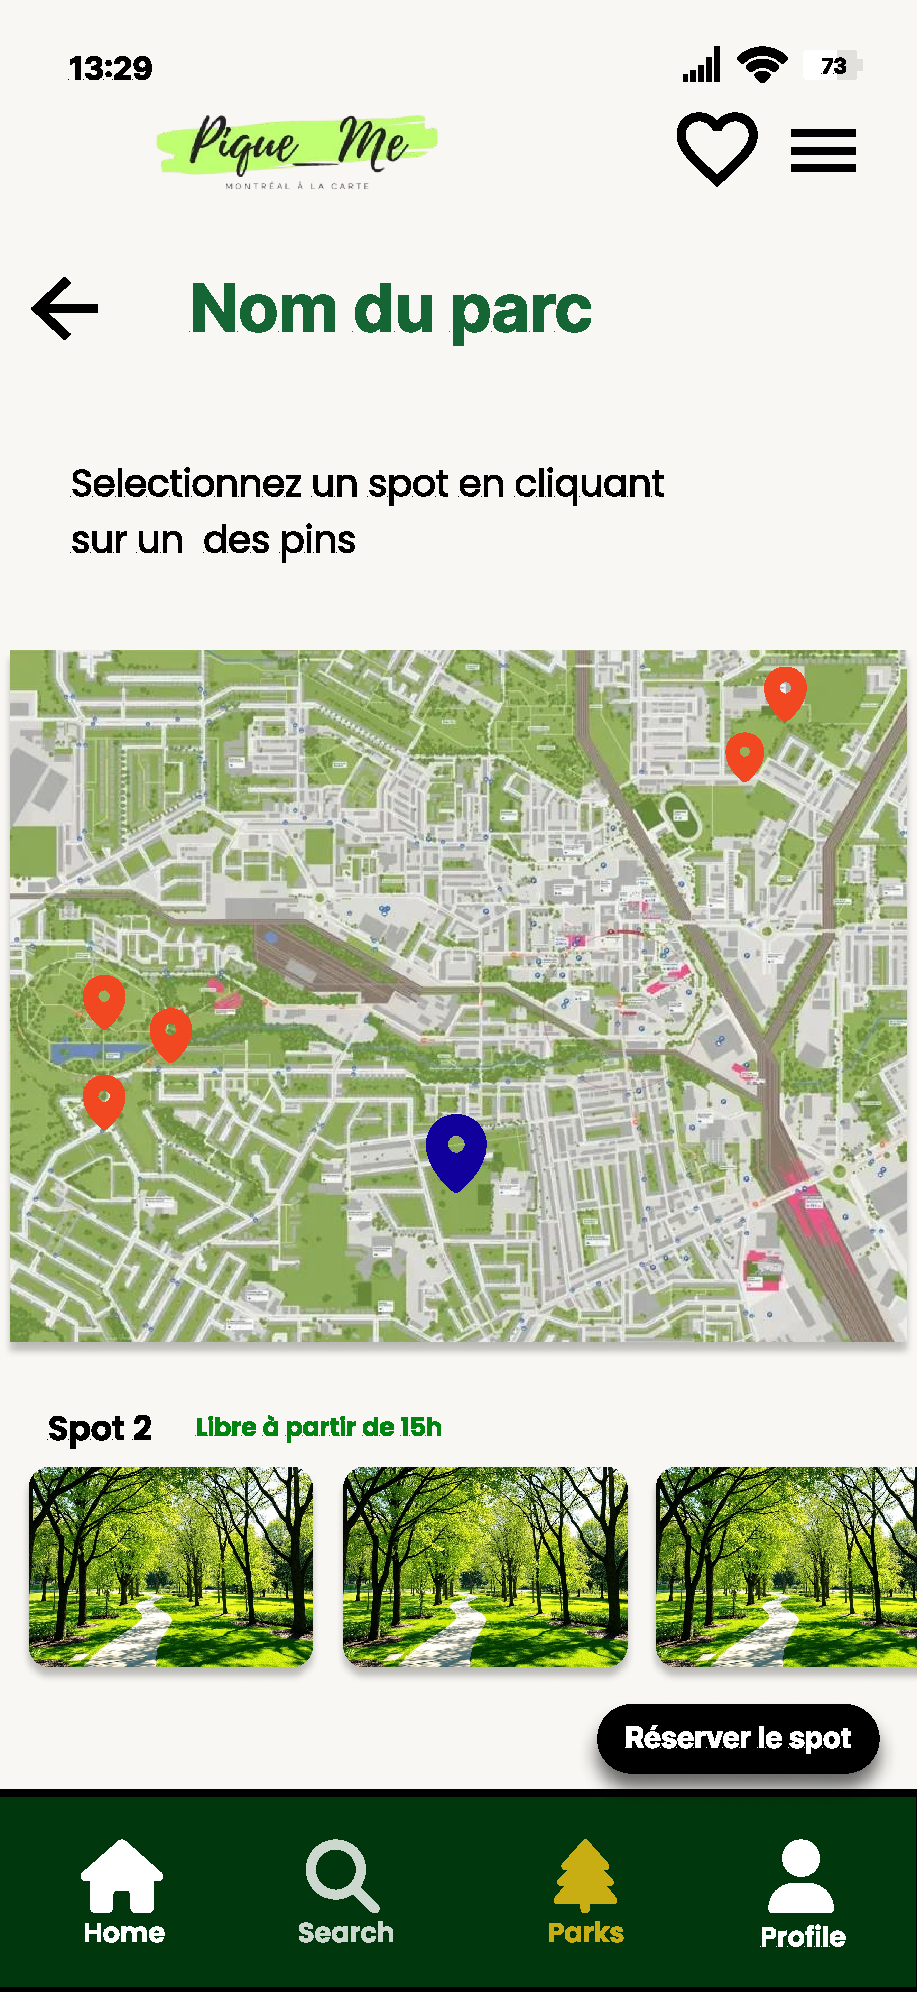
\includegraphics[width=\linewidth]{attachments/reserverSpot1.pdf}
      \caption{Choix du spot pour la réservation.}
    }
  \end{minipage}
\end{figure}

\begin{figure}[h!]
  \centering
  \begin{minipage}[t]{0.45\linewidth}
    \vtop{
      \centering
      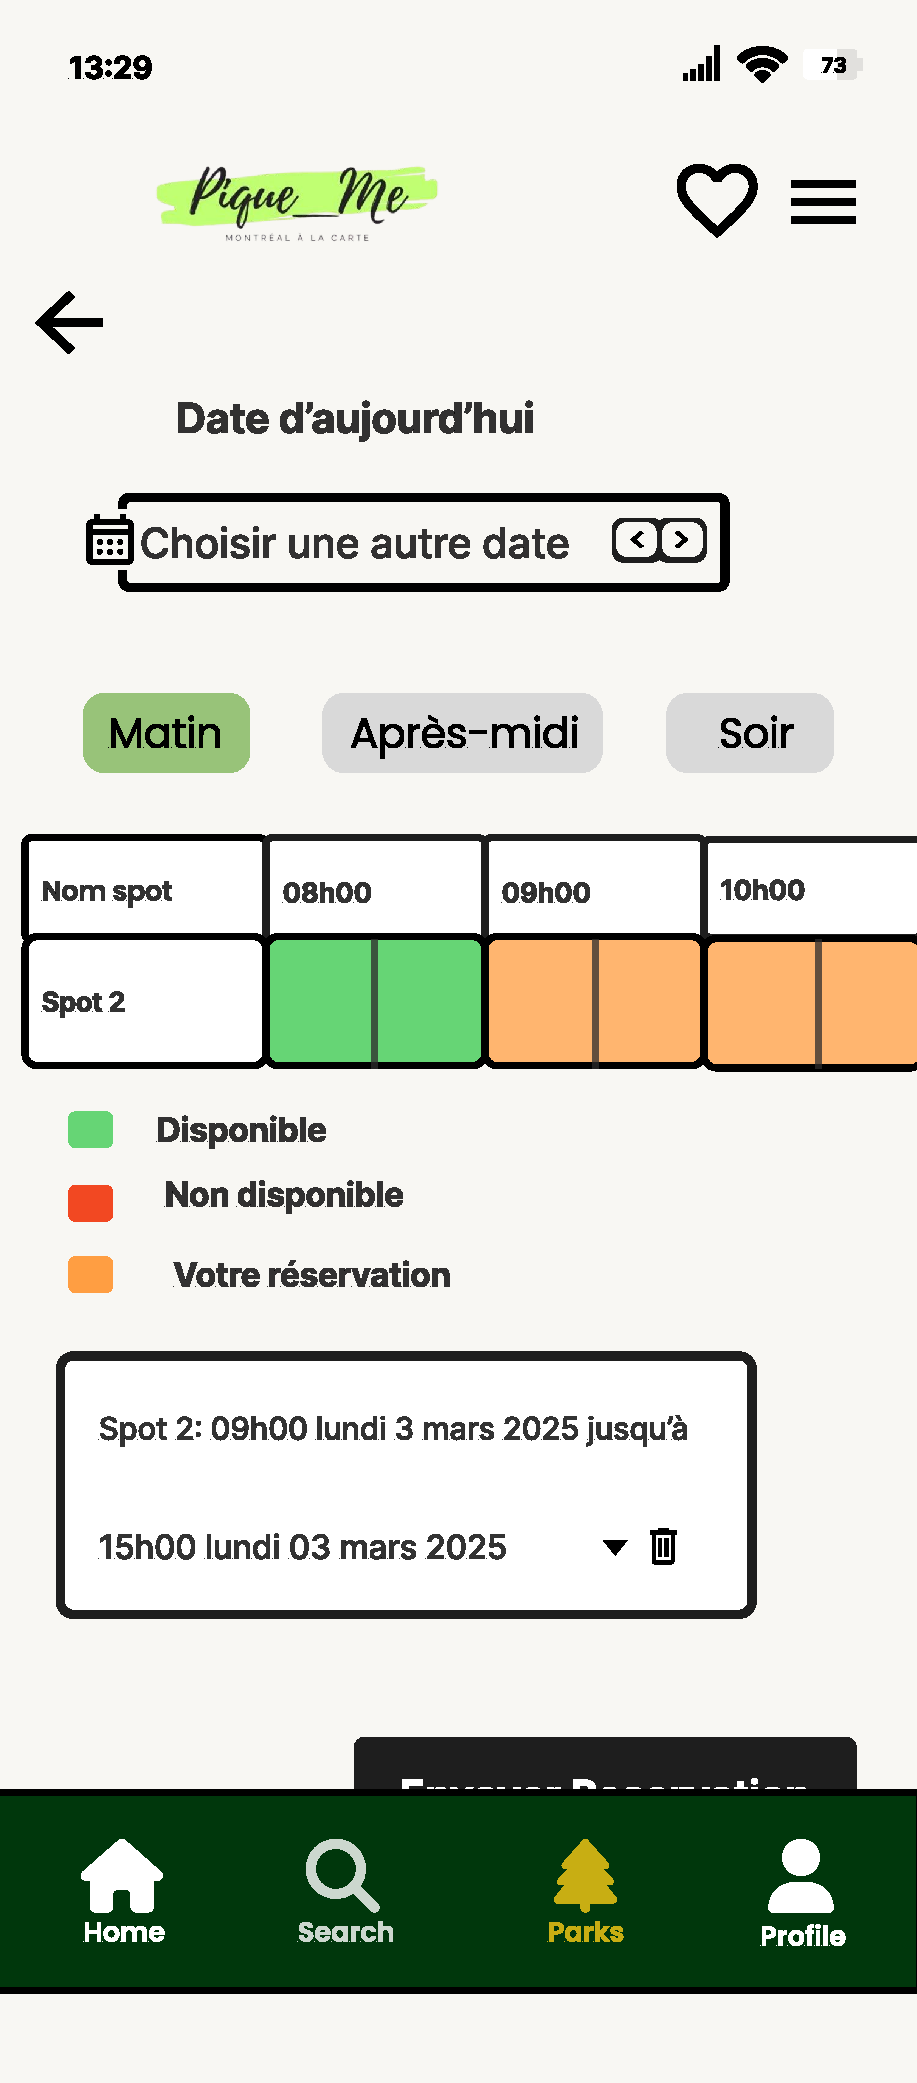
\includegraphics[width=\linewidth]{attachments/reserverSpot2.pdf}
      \caption{Choix du créneau horaire.}
    }
  \end{minipage}
  \hfill
  \begin{minipage}[t]{0.45\linewidth}
    \vtop{
      \centering
      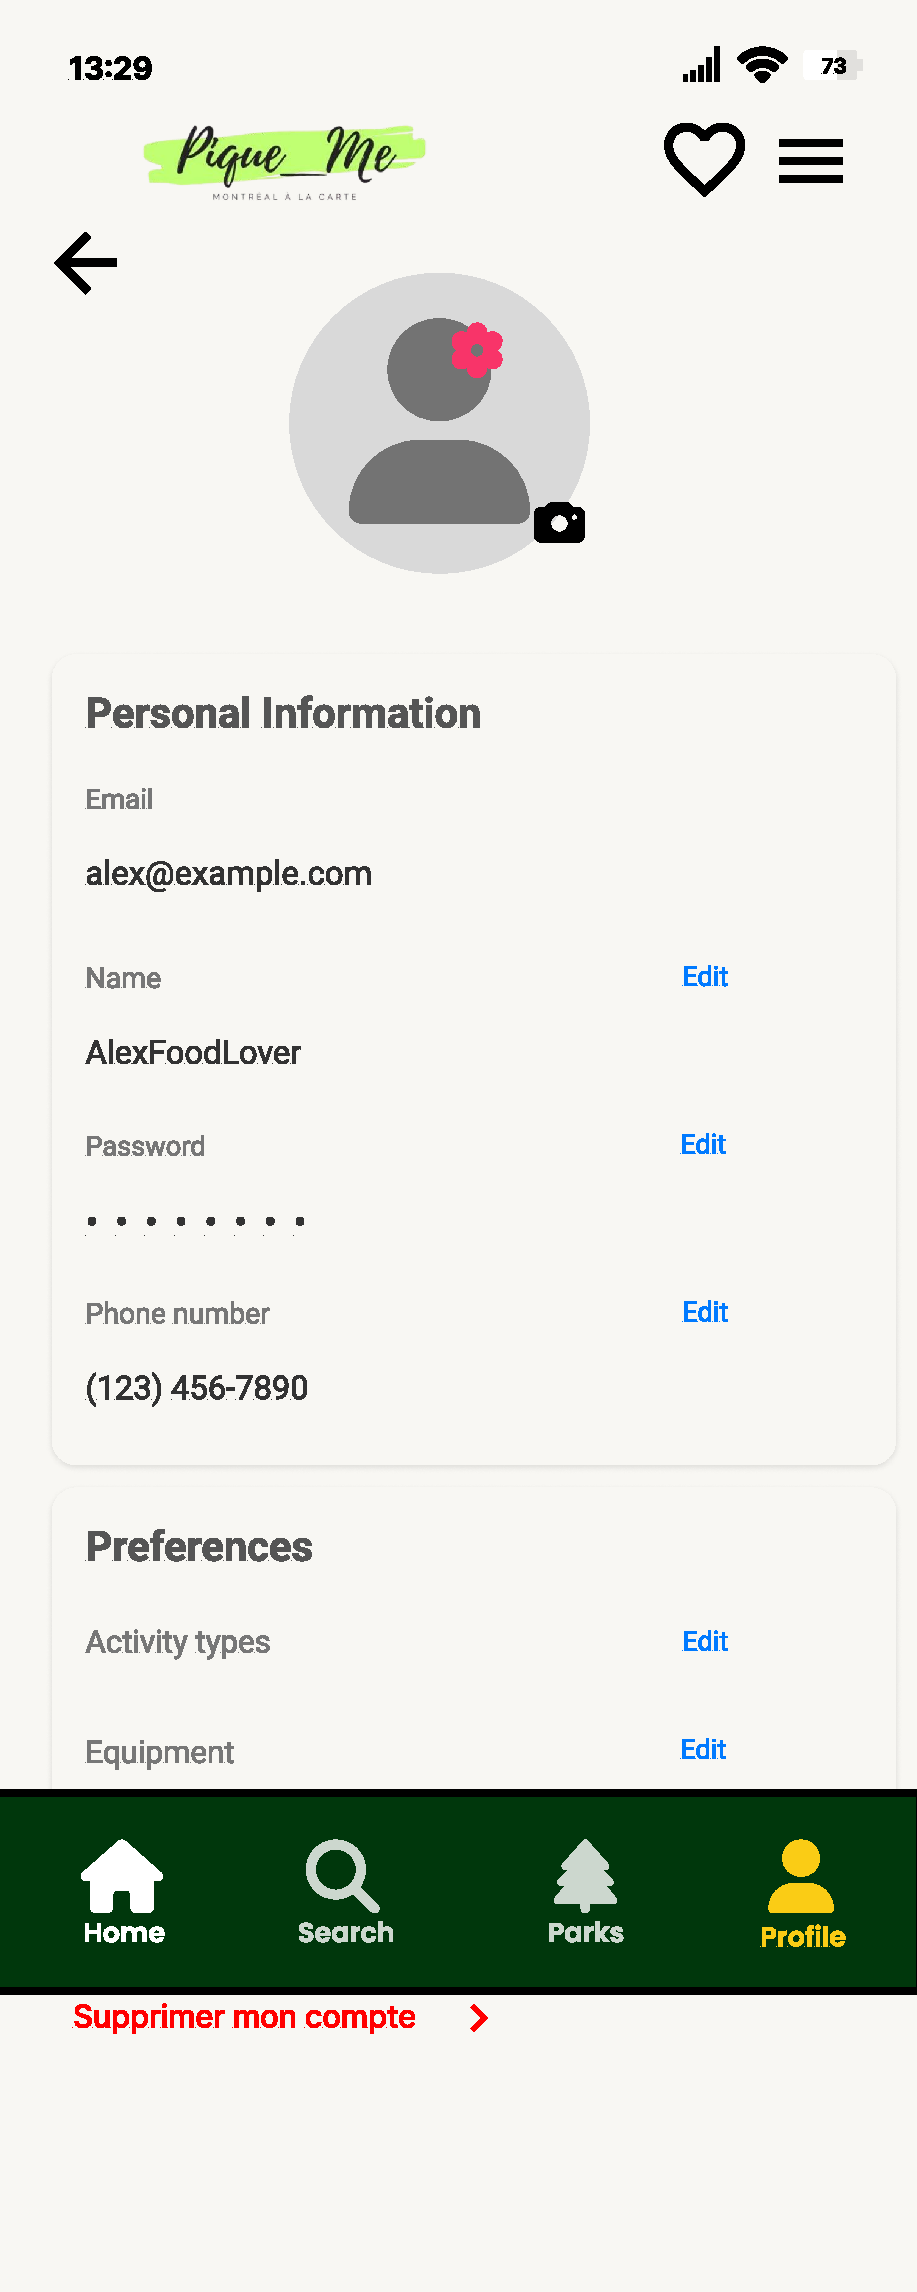
\includegraphics[width=\linewidth]{attachments/PageUser.pdf}
      \caption{Page utilisateur connecté.}
    }
  \end{minipage}
\end{figure}



\end{document}
